\documentclass[12pt,a4]{report}
\usepackage{textcomp}
\usepackage{fancyhdr}
\usepackage{graphicx}
\usepackage{titletoc,tocloft}
\usepackage{enumitem}
\usepackage{amsmath,amssymb}
\usepackage{tabularx}
\usepackage{tabularx}
\usepackage{longtable}
\usepackage{array}
\usepackage{ragged2e}
\usepackage{ltablex}
\usepackage{geometry}
\geometry{margin=1in}
\usepackage{array}
\usepackage{longtable}
\usepackage{setspace}
\usepackage{titlesec}
\usepackage{lscape}
\keepXColumns

\evensidemargin 0.5in
\oddsidemargin 0.0in
\topmargin 0.5in
\textwidth 6.5in
\headheight 0.3in
\headsep 0in

% 
\usepackage[]{hyperref}
\usepackage{tikz}
\usetikzlibrary{arrows,shapes,snakes,automata,backgrounds,petri}

\usepackage{tabularx}

\usepackage{pgfgantt}
\usepackage[margin=1in]{geometry}
\usepackage{lscape}
% \usepackage[margin=0.8in]{geometry}
\usepackage{array}
\usepackage{longtable}
\usepackage{multirow}
%\usepackage[nottoc,notlot,notlof,numbib]{tocbibind}
\usepackage[titletoc]{appendix}
% \usepackage{titletoc}
\renewcommand{\bibname}{References}
\setcounter{secnumdepth}{5}
\usepackage{float}
\usepackage{subcaption}
\usepackage{multirow}
\usepackage{longtable}
\usepackage{geometry}
\geometry{margin=1in}
\usepackage{caption}
\usepackage[ruled,vlined]{algorithm2e}
\newcommand{\cellpadding}{\renewcommand{\arraystretch}{1.2}}
\newcommand{\headerpadding}{\renewcommand{\arraystretch}{1.5}}
% Define new column type for justified text with padding
\newcolumntype{P}[1]{>{\raggedright\arraybackslash}p{#1}}
\textheight 8.5in
\newcommand{\pa}{\hspace{3ex}}
\newcommand{\be}{\begin{equation}}
\newcommand{\ee}{\end{equation}}
\newcommand{\fs}{\hspace{2ex}}
\newcommand{\no}{\noindent}
\newcommand{\hs}{\hspace{1ex}}
\newtheorem{myth}{Theorem}
\newcommand{\smci}{{\bf smci }}
\newcommand{\smcd}{{\bf smcd }}
\newcommand{\smc}{{\bf smc }}
\newcommand{\ab}{{\bf sc4c }}
\newcommand{\hub}{H\"ubler }
\newcommand{\ds}{D^m_f}
\newtheorem{prop}{Proposition}
\newtheorem{cor}{Corollary}
\newtheorem{defn}{Definition}
\newcommand{\rr}{{\cal R }^2 }
\newcommand{\zz}{{\cal Z }^2 }
\newcommand{\at}{{A_o}^T}
\newcommand{\ato}{{A_1}^T}
\newcommand{\ath}{{\at}_{\hat{h}}}
\newcommand{\ata}{\tilde{\at}}
\newcommand{\on}{(s_1,\hat{s_1}]}
\newcommand{\tw}{(\hat{s_1},b]}
\newcommand{\hb}{\hat{B}}
\newcommand{\hfo}{{\hat{f}}_1}
\newcommand{\xy}{(x,y)}
\newcommand{\txy}{(t_x,t_y)}
\renewcommand{\r}{{\cal R}}
\newcommand{\ct}{\hat{C}_1^T}
\newcommand{\xh}{X_{\hat{h}}}
\newcommand{\ball}{B((x_o,y_o),r)}
\newcommand{\snbd}{S((x_o,y_o),k)}
\newcommand{\xyo}{(x_o,y_o)}
\newtheorem{obs}{Observation}
\newtheorem{lemma}{Lemma}
\newcommand{\CC}{{\cal C }}
\newcommand{\DD}{{\cal D }}
\newcommand{\cset}{{\{C\}}}
\newcommand{\dset}{{\{D\}}}
\newcommand{\sdset}{{\sigma_{\dset}}}
\newcommand{\dsetm}{{m\dset}}
\newcommand{\sdsetm}{{\sigma_{\dsetm}}}
\newcommand{\od}{{O_D}}
\newcommand{\id}{{I_D}}
\newcommand{\ido}{{\id_1}}
\newcommand{\idt}{{\id_2}}
\newcommand{\odo}{{\od_1}}
\newcommand{\odt}{{\od_2}}
\newcommand{\rido}{{R(\ido)}}
\newcommand{\ridt}{{R(\idt)}}
\newcommand{\rodo}{{R(\odo)}}
\newcommand{\rodt}{{R(\odt)}}
\newcommand{\xe}{$x$-extent}
\newcommand{\ye}{$y$-extent}
\newcommand{\kxo}{k_{x1}}
\newcommand{\kxt}{k_{x2}}
\newcommand{\kxth}{k_{x3}}
\newcommand{\kyo}{k_{y1}}
\newcommand{\kyt}{k_{y2}}
\newcommand{\kyth}{k_{y3}}
\newcommand{\Ra}{{\Rightarrow}}
\newcommand{\is}{\Rightarrow \hspace{10mm}}
\newcommand{\vs}{\vspace{0.2in}}
\newcommand{\im}{{\lfloor m \rfloor}}
\newcommand{\fm}
\newcommand{\dm}{{\Delta m}}
\newcommand{\ic}{{\lfloor c \rfloor}}
\newcommand{\fc}
\newcommand{\dc}{{\Delta c}}
\newcommand{\yi}{{y_i}}
\renewcommand{\xi}{{x_i}}
\newcommand{\alpp}{{{\alpha}_{2}}}
\newcommand{\alp}{{{\alpha}_{1}}}
\newcommand{\bett}{{{\beta}_{2}}}
\newcommand{\bet}{{{\beta}_{1}}}
\newcommand{\lqr}{{\lfloor q \rfloor}}
\newcommand{\ramax}{R_{max}^A}
\newcommand{\ramin}{R_{min}^A}
\newtheorem{property}{Property}
\newcommand{\sla}{{{S_{\lambda}}}}
\newcommand{\vf}{{\vspace{0.50in}}}
\newcommand{\ms}{\;}
\renewcommand{\appendixname}{Annexure}

% Rename "Contents" to "INDEX"
\renewcommand{\contentsname}{INDEX}

% Disable header/footer for chapter title pages
\fancypagestyle{chaptertitle}{
  \fancyhf{} % clear all
  \renewcommand{\headrulewidth}{0pt}
  \renewcommand{\footrulewidth}{0pt}
}

% ==========================================
%  CUSTOM CHAPTER STYLE – CENTER TITLE PAGE
% ==========================================
\makeatletter
\def\@makechapterhead#1{%
  \vspace*{\fill}%
  \begin{center}
    {\Huge\bfseries CHAPTER \thechapter\\[1.5ex]#1}
  \end{center}
  \thispagestyle{chaptertitle}% disable headers/footers
  \vspace*{\fill}
  \clearpage
}
\def\@makeschapterhead#1{%
  \vspace*{\fill}%
  \begin{center}
    {\Huge\bfseries #1}
  \end{center}
  \thispagestyle{chaptertitle}%
  \vspace*{\fill}
  \clearpage
}
\makeatother

\newcommand{\createGanttChart}{%
    \begin{table}[htbp]
    \centering
    \caption{Project Timeline}
    \begingroup
    \renewcommand\sfdefault{phv}
    \renewcommand\mddefault{mc}
    \renewcommand\bfdefault{bc}
    
    \sffamily
    \begin{ganttchart}[
        % --- Chart Styling ---
        canvas/.append style={fill=none, draw=black!5, line width=.75pt},
        hgrid style/.style={draw=black!5, line width=.75pt},
        vgrid={*1{draw=black!5, line width=.75pt}},
        title/.style={draw=none, fill=none},
        title label font=\bfseries\footnotesize,
        title label node/.append style={below=7pt},
        include title in canvas=false,
        bar label font=\mdseries\small\color{black!70},
        bar label node/.append style={left=2cm},
        bar/.append style={draw=none, fill=black!63},
        bar incomplete/.append style={fill=barblue},
        bar progress label font=\mdseries\footnotesize\color{black!70},
        group incomplete/.append style={fill=groupblue},
        group left shift=0,
        group right shift=0,
        group height=.5,
        group peaks tip position=0,
        group label node/.append style={left=.6cm},
        group progress label font=\bfseries\small,
        x unit=0.7cm,
        title label node/.append style={xshift=0.1cm}
    ]{1}{12}
      % --- Titles ---
      \gantttitle[
        title label node/.append style={below left=7pt and -3pt}
      ]{2025}{12} \\
      \gantttitlelist[
        title label node/.append style={below left=7pt and -3pt}
      ]{{"Jan"}, {"Feb"}, {"Mar"}, {"Apr"}, {"May"}, {"Jun"}, {"Jul"}, {"Aug"}, {"Sep"}, {"Oct"}, {"Nov"}, {"Dec"}}{1} \\
      % --- Tasks ---
      \ganttgroup{Project Timeline}{1}{12} \\
      \ganttbar[name=planning]{\textbf{1.} Initial Planning and Requirement Gathering}{1}{2} \\
      \ganttbar[name=research]{\textbf{2.} Research and Technology Selection}{3}{4} \\
      \ganttbar[name=dataset]{\textbf{3.} Dataset Collection and Preprocessing}{5}{6} \\
      \ganttbar[name=prototype]{\textbf{4.} Prototype Development and PoC}{7}{8} \\
      \ganttbar[name=testing]{\textbf{5.} Testing and Validation}{9}{10} \\
      \ganttbar[name=implementation]{\textbf{6.} Final Implementation and Deployment}{11}{12}\\
      \ganttbar[name=documentation]{\textbf{7.} Documentation}{10}{12}
    \end{ganttchart}
    \endgroup
    
    \label{gantt:project-timeline}
    \end{table}
}
\input{psfig.sty}

\begin{document}
% ==========================================
% FIRST 2 PAGES: No headers, footers, or page numbers
% ==========================================
\pagenumbering{gobble}
\pagestyle{empty}

% Page 1: Title page
\vspace*{\fill}
\begin{center}

{\large  A  PROJECT REPORT ON}\\
\vspace{0.5cm}
\vspace{0.5cm}
{\bfseries \fontsize{16}{12} \selectfont{MolVista AI}  \\ \vspace*{1\baselineskip}}
{\bfseries \fontsize{14}{12} \selectfont{Deep Learning Based Platform for Molecular Docking and Binding Affinity Prediction}  \\ \vspace*{2\baselineskip}}
{\fontsize{12}{12} \selectfont Submitted towards the
 \\Partial Fulfilment of the Requirements of} \\
\vspace{1cm}
{\bfseries \fontsize{14}{12} \selectfont BACHELOR OF TECHNOLOGY \\
\vspace*{0.5\baselineskip}
IN
\vspace*{0.5\baselineskip}
\\ARTIFICIAL INTELLIGENCE AND DATA SCIENCE\\
\vspace*{1\baselineskip}} 
\fontsize{14}{12} \selectfont \textbf{By} \\
{\large \begin{center}
\begin{tabular}{l l}
Shreeyan Manoj Patil        & Examination Seat No: B221311090  \\
Swarali Prashant Bedse        & Examination Seat No: B221311007  \\
Rajesh Bhagvan Khavane            & Examination Seat No: B221311063 \\
Prasad Bharat Lonare        & Examination Seat No: B221311068  \\

\end{tabular}
\end{center}}
{\bfseries \large Under the guidance of} \\
\vspace{0.5cm}
{\bfseries \large Dr. S. A. Khaire} \\ \vspace{0.5cm}

\begin{figure}[!h]
\centering
  
\includegraphics[width=1.5in]{KKWLOGO.v1.jpg}
\end{figure}


{\small Department of Artificial Intelligence and Data Science}\\
\fontsize{13}{13} \selectfont K. K. WAGH EDUCATION SOCIETY\textquotesingle S\\
\fontsize{13}{13} \selectfont K. K. WAGH INSTITUTE OF ENGINEERING EDUCATION AND RESEARCH\\
Hirabai Haridas Vidyanagari, Amrutdham, Panchavati, Nashik, Maharashtra 422003 \\
(An Autonomous Institute since 2022, affiliated to Savitribai Phule Pune University)\\
A. Y. 2025-2026
\vspace*{\fill}
\end{center}

\pagebreak

% Page 2: Certificate
% \begin{figure}[!h]
% \centering
%   \includegraphics[width=1.9in]{Logo.png}
% \end{figure}

% \begin{center}
% % {\small Department of Artificial Intelligence and Data Science}\\
% % K. K. WAGH EDUCATION SOCIETY\textquotesingle S\\
% % K. K. WAGH INSTITUTE OF ENGINEERING EDUCATION AND RESEARCH\\
% % Hirabai Haridas Vidyanagari, Amrutdham, Panchavati, Nashik, Maharashtra 422003 \\
% % (An Autonomous Institute affiliated to Savitribai Phule Pune University)\\	
% {\small Department of Artificial Intelligence and Data Science }\\
% K. K. WAGH EDUCATION SOCIETY\textquotesingle S\\
% K. K. WAGH INSTITUTE OF ENGINEERING EDUCATION AND RESEARCH\\
% (An Autonomous Institute affiliated to Savitribai Phule Pune University)\\	
% \vspace{0.5cm}
% {\Large \bf{CERTIFICATE}} \\ \vspace{0.5cm}

% \end{center}

% \centerline{This is to certify that the project report entitled}
% \vspace*{1\baselineskip} 

% {\bfseries \fontsize{16}{12} \centering\selectfont{PolicyVault Nexus}  \\ \vspace*{1\baselineskip}}
% {\bfseries \fontsize{13}{12} \centering\selectfont{Responsible Data Sharing in Fintech Enviornment}  \\ \vspace*{1\baselineskip}}

% \centerline{being submitted by} 
% {\large \begin{center}
% \begin{tabular}{l l}
% Rasika Santosh Thakur        & Examination Seat No: B221311136 \\
% Varad Sandeep Joshi            & Examination Seat No: B221311051 \\
% Soham Ainath Penshanwar        & Examination Seat No: B221311104 \\
% \end{tabular}
% \end{center}}
% \vspace*{1\baselineskip} 
% is a bonafide work carried out by them under the supervision of Dr. S. A. Khaire and it is approved for the partial fulfilment of the requirement of Bachelor of Technology (Artificial Intelligence and Data Science) during Academic Year 2025-2026.
% \vspace*{1\baselineskip}
% \\This project report has not been earlier submitted to any other Institute or University for the award of any degree or diploma.
% \vspace*{1\baselineskip}

% \bgroup
% \def\arraystretch{0.7}
% \noindent
% \makebox[\textwidth][s]{%
%     \begin{minipage}[t]{0.45\textwidth}
%         \centering
%         Dr. S. A. Khaire \\
%         Internal Guide \\
%         Department of \\
%         Artificial Intelligence and Data Science
%     \end{minipage}%
%     \hfill
%     \begin{minipage}[t]{0.45\textwidth}
%         \centering
%         Prof. Dr. S. M. Kamalapur \\
%         Head, \\
%         Department of \\
%         Artificial Intelligence and Data Science
%     \end{minipage}
% }
% \egroup

% \vspace*{3\baselineskip} % 3 lines space

% \begin{flushleft}
% External Examiner

% \vspace*{1\baselineskip} % 2 lines space

% Date: \\
% Place: Nashik
% \end{flushleft}

% \begin{figure}[!h]
% \centering
%   
\includegraphics[width=1.6in]{KKWLOGO.v1.jpg} % Reduced slightly
%   \vspace{-0.8cm}
% \end{figure}

\begin{center}
% {\small Department of Artificial Intelligence and Data Science }\\
% K. K. WAGH EDUCATION SOCIETY\textquotesingle S\\
% K. K. WAGH INSTITUTE OF ENGINEERING EDUCATION AND RESEARCH\\
% (An Autonomous Institute affiliated to Savitribai Phule Pune University)\\	
\vspace*{3\baselineskip} % Reduced
{\Large \bf{CERTIFICATE}} \\
% \vspace{0.3cm}
\end{center}

\vspace{0.4cm}
\centerline{\textit{This is to certify that the project report entitled}}
\vspace*{0.6\baselineskip} % Reduced

{\bfseries \fontsize{16}{12} \centering\selectfont{MolVista AI}  \\}
\vspace*{0.3\baselineskip} % Reduced
{\bfseries \fontsize{14}{12} \centering\selectfont{Deep Learning Based Platform for Molecular Docking and Binding Affinity Prediction}  \\}
\vspace*{0.6\baselineskip} % Reduced

\centerline{\textit{being submitted by}} 
\vspace*{0.5\baselineskip} % Reduced

{\large \begin{center}
\begin{tabular}{l l}
Shreeyan Manoj Patil        & Examination Seat No: B221311090  \\
Swarali Prashant Bedse        & Examination Seat No: B221311007  \\
Rajesh Bhagvan Khavane            & Examination Seat No: B221311063 \\
Prasad Bharat Lonare        & Examination Seat No: B221311068  \\
\end{tabular}
\end{center}}

\vspace*{1.5\baselineskip} % Reduced
\noindent is a bonafide work carried out by them under the supervision of Dr. S. A. Khaire and it is approved for the partial fulfilment of the requirement of Bachelor of Technology (Artificial Intelligence and Data Science) during academic Year 2025-2026.

\vspace*{0.8\baselineskip} % Reduced
\noindent This project report has not been earlier submitted to any other Institute or University for the award of any degree or diploma.

\vspace*{3.5\baselineskip} % Slightly reduced

\bgroup
\def\arraystretch{0.7}
\noindent
\makebox[\textwidth][s]{%
    \begin{minipage}[t]{0.45\textwidth}
        % \centering
        \begin{flushleft}
        \textbf{Dr. S. A. Khaire} \\
        Internal Guide \\
        % Department of \\
        % Artificial Intelligence and Data Science
        \end{flushleft}
        
    \end{minipage}%
    \hfill
    \begin{minipage}[t]{0.45\textwidth}
        % \centering
        \begin{flushright}
        \textbf{Prof. Dr. S. M. Kamalapur} \\
        Head of Department, \\
        Department of AI\&DS \\
        
        \end{flushright}
        
    \end{minipage}
}
\egroup

% \bgroup
% \def\arraystretch{0.7}
% \noindent
% \makebox[\textwidth][s]{%
%     \begin{minipage}[t]{0.45\textwidth}
%         \centering
        
%         \textbf{Dr. S. A. Khaire} \\
%         Internal Guide \\
%         Department of \\
%         Artificial Intelligence and Data Science
%     \end{minipage}%
%     \hfill
%     \begin{minipage}[t]{0.45\textwidth}
%         \centering
        
%         \textbf{Prof. Dr. S. M. Kamalapur} \\
%         Head, \\
%         Department of \\
%         Artificial Intelligence and Data Science
%     \end{minipage}
% }
% \egroup

\vspace*{2.5\baselineskip} % Reduced from 3

\begin{flushleft}

\textbf{External Examiner}\\
\vspace*{2.5\baselineskip}
\textbf{Date: }22-11-2025\\
\textbf{Place: }Nashik
\end{flushleft}

\vspace*{1.5\baselineskip}

% \noindent\textbf{Date: }DD-MM-YYYY \hfill \textbf{Place: }Nashik

% \begin{figure}[!h]
% \centering
%   \includegraphics[width=1.6in]{Logo.png} % Reduced slightly
%   \vspace{-0.8cm}
% \end{figure}

% \begin{center}
% % {\small Department of Artificial Intelligence and Data Science }\\
% % K. K. WAGH EDUCATION SOCIETY\textquotesingle S\\
% % K. K. WAGH INSTITUTE OF ENGINEERING EDUCATION AND RESEARCH\\
% % (An Autonomous Institute affiliated to Savitribai Phule Pune University)\\	
% \vspace{0.5cm} % Reduced
% {\Large \bf{CERTIFICATE}} \\
% \vspace{0.1cm} % Reduced
% \end{center}

% \centerline{This is to certify that the project report entitled}
% \vspace*{0.5\baselineskip} % Reduced

% {\bfseries \fontsize{16}{12} \centering\selectfont{PolicyVault Nexus}  \\}
% \vspace*{0.6\baselineskip} % Reduced
% {\bfseries \fontsize{14}{12} \centering\selectfont{Responsible Data Sharing in Fintech Enviornment}  \\}
% \vspace*{0.6\baselineskip} % Reduced

% \centerline{being submitted by} 
% \vspace*{0.5\baselineskip} % Reduced

% {\large \begin{center}
% \begin{tabular}{l l}
% Rasika Santosh Thakur        & Examination Seat No: B221311136 \\
% Varad Sandeep Joshi          & Examination Seat No: B221311052 \\
% Soham Ainath Penshanwar      & Examination Seat No: B221311104 \\
% \end{tabular}
% \end{center}}

% \vspace*{0.5\baselineskip} % Reduced
% is a bonafide work carried out by them under the supervision of Dr. S. A. Khaire and it is approved for the partial fulfilment of the requirement of Bachelor of Technology (Artificial Intelligence and Data Science) during Academic Year 2025-2026.

% \vspace*{0.5\baselineskip} % Reduced
% This project report has not been earlier submitted to any other Institute or University for the award of any degree or diploma.

% \vspace*{2\baselineskip} % Slightly reduced

% \bgroup
% \def\arraystretch{0.7}
% \noindent
% \makebox[\textwidth][s]{%
%     \begin{minipage}[t]{0.45\textwidth}
%         \centering
%         \textbf{Dr. S. A. Khaire} \\
%         Internal Guide \\
%         Department of \\
%         Artificial Intelligence and Data Science
%     \end{minipage}%
%     \hfill
%     \begin{minipage}[t]{0.45\textwidth}
%         \centering
%         \textbf{Prof. Dr. S. M. Kamalapur} \\
%         Head, \\
%         Department of \\
%         Artificial Intelligence and Data Science
%     \end{minipage}
% }
% \egroup

% \vspace*{1.8\baselineskip} % Reduced from 3

% % \begin{flushleft}
% % \textbf{External Examiner} \\[1\baselineskip] % Was 2 lines
% \begin{center}
% \textbf{External Examiner}
% \end{center}

% % \begin{flushleft}
% % \textbf{Date:} dd-mm-yyyy \\
% % \textbf{Place:} Nashik
% % \end{flushleft}

% \noindent\textbf{Date: }dd-mm-yyyy \hfill \textbf{Place: }Nashik

\pagebreak

% ==========================================
% ROMAN NUMBERING SECTION: Pages with roman numerals at bottom center
% ==========================================
\pagenumbering{Roman}
\setcounter{page}{1}

% Define a page style for roman numbered pages with centered footer
\fancypagestyle{romanpages}{
  \fancyhf{} % clear all
  \fancyfoot[C]{\thepage} % centered page number in footer
  \renewcommand{\headrulewidth}{0pt}
  \renewcommand{\footrulewidth}{0pt}
}

% Page I: Abstract
\pagestyle{romanpages}
\begin{center}
\bfseries \fontsize{24}{12} \selectfont Abstract
\end{center}
\vspace*{1\baselineskip}

\noindent Computational drug discovery has big problems because traditional \textbf{molecular docking} methods take a lot of time and use a lot of computer power. These old methods usually rely on \textbf{fixed energy scoring} and check every possible way a molecule can fit, which makes them slow and not very accurate. To fix these issues, we created \textbf{MolVista AI}, a smart system that uses \textbf{geometric deep learning} and \textbf{neural interaction models} to predict how molecules bind and how strong that binding is. Our system uses \textbf{SE(3)-equivariant graph neural networks} to predict where a drug molecule might fit into a target protein, keeping things the same even if the shape is rotated or moved. It also includes a \textbf{Neural Affinity Predictor} that looks at features like distances between atoms, angles, and contact maps to estimate how strong the binding is. \textbf{MolVista AI} is a complete system that can automatically prepare data, predict how a molecule will fit, and rate how strong the binding is, all in one process. The platform works with common file formats like \textbf{PDB}, \textbf{SDF}, and \textbf{MOL2}, making it easy to use with existing tools in the field. When we tested MolVista AI on the \textbf{PDBbind v2020} dataset, it performed very well, predicting accurate docking positions with an average \textbf{RMSD of 3.48 angstroms} and a \textbf{correlation coefficient of 0.89} with real experimental data. Additionally, it operates faster than conventional techniques, processing each molecule complex on a GPU in just \textbf{0.3 seconds}. A wide range of people can now access sophisticated docking tools thanks to \textbf{MolVista AI}'s web-based interface, which allows users to view molecules in real time, perform batch analyses, and download comprehensive results. By combining \textbf{geometric deep learning}, \textbf{neural scoring}, and \textbf{web technology}, MolVista AI sets a new standard for \textbf{AI-based molecular docking}. It helps speed up early drug discovery and improves the clarity and reliability of research on molecular interactions.

\vspace{\baselineskip}
\noindent \textbf{Keywords: } \textit{Geometric Deep Learning, SE(3)-Equivariant Graph Neural Network, Binding Affinity Prediction, Molecular Docking, Protein–Ligand Interaction, Computational Drug Discovery, Artificial Intelligence, Structural Bioinformatics}

\pagebreak


% Page II: Acknowledgement
\begin{center}
\bfseries \fontsize{24}{12} \selectfont Acknowledgement
\end{center}
\vspace*{1\baselineskip}
\hspace*{0.5in}We would like to thank our project guide, Dr. S. A. Khaire, for her guidance and support. We will forever remain grateful for the constant encouragement and assistance extended by our guide in making this Project Phase II report. Through our many discussions, she helped us to form and solidify ideas. The invaluable discussions we had with her and our team colleagues, the penetrating questions she posed to us, and her constant motivation have all led to the development of the ideas presented in this Project Phase II report. We would also like to express our sincere gratitude to our Departmental Co-ordinator of Artificial Intelligence and Data Science, Dr. D. V. Medhane, and our esteemed Director, Dr. K. N. Nandurkar, for their continued support and leadership. Furthermore, we thank our sponsorship agency for their generous assistance, which greatly facilitated the completion of this work.\

\hspace*{0.5in}We would also like to thank our wonderful colleagues, parents, and friends for listening to our ideas, asking questions, and providing feedback and suggestions for improving our ideas.\\

\vspace*{3\baselineskip} 
% \begin{tabular}{p{8.2cm}c}
% &
% %}
% \end{tabular}
\begin{flushright}
Prasad Bharat Lonare \\
Rajesh Bhagvan Khavane \\
Shreeyan Manoj Patil \\
Swarali Prashant Bedse
\end{flushright}

\bibliographystyle{plain}
\newpage

% Page III: INDEX (Table of Contents) - no header/footer on any page
\pagestyle{romanpages}
\tableofcontents
\addtocontents{toc}{\protect\thispagestyle{romanpages}}

\let\origaddvspace\addvspace
\renewcommand{\addvspace}[1]{}

% Page IV: List of Tables - no header/footer
\clearpage
\pagestyle{romanpages}
	% \addcontentsline{toc}{section}{\bf LIST OF TABLES}
	\setcounter{lotdepth}{2} 
\listoftables
\addtocontents{lot}{\protect\thispagestyle{romanpages}}

% Page V: List of Figures - no header/footer
\clearpage
\pagestyle{romanpages}
	% \addcontentsline{toc}{section}{\bf LIST OF FIGURES}
	\setcounter{lofdepth}{2} 
\listoffigures
\addtocontents{lof}{\protect\thispagestyle{romanpages}}

% ==========================================
% START OF CHAPTERS: Arabic page numbering begins
% ==========================================
\clearpage
\pagenumbering{arabic}
\setcounter{page}{1}

\fancyhf{}
% \rhead{Chapter: \thechapter}
\renewcommand{\footrulewidth}{0.4pt}
\lfoot{KKWIEER, Department of Artificial Intelligence and Data Science,2025}
\rfoot{Page \thepage}

\fancypagestyle{plain}{ % Redefine 'plain' style used by chapters
    \fancyhf{} % Clear all header and footer fields
    % \rhead{Chapter: \thechapter}
    % \renewcommand{\footrulewidth}{0.4pt}
    \lfoot{KKWIEER, Department of Artificial Intelligence and Data Science}
    \rfoot{Page \thepage}
    \renewcommand{\headrulewidth}{0.0pt} % No header rule
    \renewcommand{\footrulewidth}{0.0pt} % Keep footer rule
}
\pagestyle{fancy}

\setlength{\parindent}{11mm}



\chapter{INTRODUCTION}
\hspace*{0.3in}Discovery of drugs is a fast growing field but scientists are still encountering big challenges during the study of molecular interactions. Conventional computational tools are scientifically reliable though most of the time they require high processing power, lengthy execution time, and manual setup. A common laboratory has hundreds of chemical compounds that could be required to be analyzed on a daily basis. A number of individual software systems, reconfiguration and parameter tuning are usually associated with each analysis. The discrepancies that are present would cause researchers to re-test, compare, and manually perform every step, which is time-constraining and tedious because it is time-consuming and usually fragmented. This complication is intensifying scaling of both academic and industry groups in their research.
\\\\
\hspace*{0.3in}MolVista AI presents a new, modern, AI-based platform that is used to make predictions of protein-ligand interactions easily and faster. The platform is automated to predict binding strength with better accuracy and speed using advanced geometric deep learning and 3D structural analysis to automate docking simulations. MolVista AI provides a streamlined and seamless experience by providing the tools of molecular preparation, real-time visualization, and AI-based docking in one, well-designed web interface.
\\\\
\hspace*{0.3in}The system directs the users along smartly foretold pipeline foresight, minimizes human intervention, and holds the results consistent and simple to identify. Docking results are shown in real time in form of a dashboard with actually predicted affinities and automated preprocessing so that the molecular files are already prepared by the time the analysis commences. Practically, MolVista AI will help decrease the docking time almost by 80 percent, as the AI-improved insights are reliable to help identify potential drug candidates faster. In this introduction, this platform has been described with some of its most important functionalities based on the elements of molecular preparation, AI-based docking prediction, 3D visualization capabilities, and system evaluation procedures.\\\\

\section{Project Idea}
\hspace*{0.3in}Recent advances in computational biology/artificial intelligence is transforming the manner in which novel medications are made. Classical approaches to the modeling of protein-ligand interactions are based on physics-related simulations and usually require a significant amount of time and computer resources. Individual molecular interaction can take many minutes, hours to evaluate and this slows down large-scale screening and rapid lead discovery. With more data-intensive research, the rapidity and precision of predictions demanded using AI-capable tools are intensely sought.
\\\\
\hspace*{0.3in}MolVista AI is a designed high-tech docking platform based on geometric deep learning. It is an SE(3)-equivariant Graph Neural Networks (GNN) that can conceptualize the spatial arrangement of molecules, which in turn allow the system to learn the relationship between atoms to each other in 3D space. The model is used to predict the position of the ligands in the active site of a protein, and the probable binding affinity is estimated. Since it is informed by experimentally verified structural data, it gives resource efficient and high-quality predictions compared to classical grid-search methods or physics-only.
\\\\
\hspace*{0.3in}The system provides a full artificial intelligence docking process. The molecular structures can be uploaded as in the form of either \texttt.pdb, \texttt.sdf, and mol2. MolVista AI authentically validates the input, creates graph-based consensus, makes poses annotations, and visualizes the findings in an interactive 3D environment. It also produces affinity scores, which is a rapid and scalable alternative to the conventional docking pipelines.
\\\\
In order to fulfill these capabilities, MolVista AI uses a number of current computational techniques:
\begin{itemize}
    \item \textbf{Geometric Deep Learning:} GNNs with optimal SE(3) symmetry are employed, which preserves the physical symmetry of the three-dimensional space, and to make predictions not dependent on rotation and translation.
    \item \textbf{Short-Univariate Neural Affinity Estimation:} A deep learning model uses and compares chemical, spatial, and geometric features to predict protein-ligand binding strength.
    \item \textbf{Feature Processing and Feature Generation::} Processes ordinance checking, options extraction, and graph development at high intensity and extensive research.
    \item \textbf{3D Visualization and Interaction:} Incorporates projects such as 3Dmol.js so as to enable the user to view the predicted poses, search it, as well as export the results available in several different forms.\\
\end{itemize}

\hspace*{0.3in}MolVista AI is an efficient design that is designed to be modular and can be deployed to actual research settings. It connects scholarly creativity with medical practice in the development of biotechnology and pharmaceutical products. The platform helps researchers and computational science scientists to carry out the vast docking experiments with more accuracy, low computing cost, and accessibility. MolVista AI can integrate with any workflow regardless of whether the organization provides cloud-based or local services.\\\\
\hspace*{0.3in}MolVista AI With the addition of AI-guided automation to the intricate nature of the molecular docking work, MolVista AI provides a new data-driven structural prediction. This makes molecular modeling much less time-intensive and more reliable, which will eventually allow the process of new therapeutic candidates discovery to be faster and lead to the progress of AI in drug development.
\\\\


\section{Motivation of the Project}


\hspace{0.3in}MolVista AI has been driven by many years of difficulties in computational drug discovery and molecular docking. Despite the numerous types of docking tools, they often are faced with such problems as slow processing time, low precision, and inability to process large amounts of data. The increased access to structural data and the development of AI and geometric deep learning is one opportunity to address these constraints and bring about more efficient and stable molecular prediction frameworks.\\

\begin{enumerate}
    \item \textbf{Reducing Computational Overhead:} Current docking approaches rely on the computationally intensive nature of the energy computations and optimization steps that usually slows down the analyses. This process is highly accelerated using MolVista AI with SE(3)-equivariant GNNs which interpret 3D molecular data in a cost-effective manner.\\

    \item \textbf{Incorrectly predicting Interaction Rules:} Classical scoring functions have the tendency to simplify the rules of interaction among molecules thus making bad predictions of interactions. The MolVista AI better predicts using personalized data-driven affinity models that utilize a wider spectrum of data of chemical and spatial characteristics.\\

    \item \textbf{Integrating AI with Structural Data:} You need AI to match the physical behaviour of biomolecules. MolVista AI satisfies this requirement by using geometric deep learning schemes which are inherently sensitive to molecular structure.\\

    \item \textbf{Accelerating Early Drug Screening:} The screening of thousands of ligands is an essential part of drug discovery, thus the speed of prediction is needed. MolVista AI speeds up this procedure because it provides quick docking and affinity of high-throughput screening.\\

    \item \textbf{Enhancing Adaptability:} Most of the currently available docking reagents are effective with only a few proteins or classes of chemicals. Compared to OpenEff, trained on a variety of structural databases, MolVista AI generalizes itself more on a vast range of different molecular systems.\\

    \item \textbf{Provision of Real-Time Interactivity:} Interactive visualization features of the platform enable researchers to accommodate dynamically the world of predictions, which enhances their interpretability and general usefulness.\\

    \item \textbf{Minimizing a Manual Processing:} Conventional workflows involve time-consuming preprocessing and changes which have to be done manually on a periodical basis. MolVista AI automates such processes and decreases errors and optimizes the overall docking process.\\

    
\end{enumerate}

\hspace{0.3in}Overall, the rationale behind the development of MolVista AI is to develop a unified, intelligent, and accessible platform improving the precision, speed, and intuition of molecular docking. The project of integrating the geometric deep learning and neural affinity prediction aims to further the computational drug discovery and make AI-directed molecular research more efficient and accessible.

\chapter{LITERATURE SURVEY}
\hspace{0.3in}Major advances of artificial intelligent have significantly altered the future of computational chemistry. Scoring formulas based on physics alone, along with labor-intensive conformational searches have been used in routine to carry out tasks traditionally, bioinspiration: Molecular docking, drug-likeness and initial drug design are being revisited in their new, data-driven form. Classical workflows tended to scale poorly in terms of resource and complexity to exploit the increasing volume and complexity of current chemical libraries but AI systems that can learn directly by observing interaction patterns revealed in structurally and biochemical data have already starting to overcome this barrier. Many recent papers also highlight how generative models and scale AI systems are transforming the approaches implemented in the entire process of computational drug discovery \cite{potineni2025generative, das2025precision}.\\

\hspace{0.3in}The first basis of structure-based virtual screening was historically carried out by docking algorithms. Their capability was, however, often limited by their inability to simulate molecular flexibility, dynamic protein environments and high-throughput screening environments. Modern-day reviews suggest that although traditional docking can still be used to derive the hypothesis of working with the first hypotheses, it is more effective to complement such approaches with machine learning, resulting in significant gains in accuracy and performance in calculation time clusters \cite{vlasiou2024molecular, pinzi2019molecular}. This is a more general change regarding the adoption of entirely physics-based approaches to hybrid, flexible, and scalable pipelines.\\

\hspace{0.3in}This change has been driven by even deeper marginal cases with deep learning which allows more multidimensional representations of molecules. Rather than depending on only handcrafted features, neural networks trained on curated structural data have now the ability to learn patterns that are used to predict protein-ligand interactions, and generate meaningful embeddings that are useful in the task of, e.g., pose prediction, estimating binding affinity, and generative molecular design, among others, as well as on curated structural data \cite{odah2025ai}. These developments are the basis of such systems as MolVista AI, which is based on learned descriptors as opposed to the conventional rule-based scoring schemes.\\

\hspace{0.3in}Minimization of human inputs in the docking processes through the incorporation of AI also increased the reliability of pose generation and has resulted in high faster generation. Big-docking systems, including RapidDock which is now named as FabIndustries Web Solutions Limited scales to 3000 scaling and 6 scaling devices; RapidDock \cite{powalski2024rapiddock} and FABind \cite{gao2024fabind}  are large docking systems that use enhanced sampling, refined pocket analysis, and high-speed evaluation modules to have proteome-wide docking at lower computational cost. Other studies depict the scheme of linking the elements of predictive learning directly into the docking pipelines to instantly improve the true outcome without affecting the throughput. The developments are much in line with the objective of MolVista AI to offer quality predictions at well achievable computational speeds.\\

\hspace{0.3in}The same has been true of binding affinity prediction. Gradually, machine-learning-based scoring models, which are trained on experimental binding measurements, are performing better than the already fixed physics-based scoring functions simply because, most structural contexts and learned patterns of interaction is better represented by machine-learning functionalities \cite{borah2024aipowered}. This strategy is followed in MolVista AI through integrating pose generation and affinity scoring and reducing cases of inconsistencies common when the functions are isolated in other tools.\\

\hspace{0.3in}Other developments such as molecular representation learning and generative chemistry have extended the abilities of drug-design systems even more. It is possible to generate artificial and synthetically viable compounds, optimize aspects of physicochemical behavior, and create an individual distinct design of molecules to target a direction and particular protein antigen using generative AI methods\cite{potineni2025generative, das2025precision}. Generative AI can research novel and synthetically viable compounds, refine physicochemical properties, and customize molecule structure to a particular direction and specific protein antigen of interest using algorithmic methods of generativity AI advances management approaches and strategies to enhance existing effects and functions through additional mechanisms and possibilities of context-specific customized design models to desired The significant features of flexible and transferable molecular encoders, noted by these advances, represent core values that are encountered in the design of MolVista AI.\\

\hspace{0.3in}Parallel In tandem with this, current computers and computing platforms are more and more concerned with automation, scaling, and human-centered design. AIDDISON, released under the Apache License, as AIDDISON \cite{rusinko2023aiddison} or as PyRMD2Dock \cite{roggia2023pyrmd2dock}  experiences the use of cloud-based computation, automated preprocessing, combined validation, accessible interfaces to smooth formulate the entire docking pipeline. The trends indicated an increased desire to have systems which provide scientific accuracy and at the same time are easily usable. The MolVista AI is a direct response to this need where complex computational routines and a web based environment have been offered to enable easier workflow.\\

\hspace{0.3in}Nevertheless, there are still a number of challenges despite this momentum. There are still a lot of AI-based frameworks with slowness in inference, lack of interpretability, or challenges going between academic prototyping and a work tool. The current systems usually focus on the improvement of algorithms without entirely incorporating docking, scoring, visualizing, and user experience. MolVista AI will solve these problems with geometrical deep learning, co-learned predictive models, automatic data management, and interactive visualization orchestrated in a production model.\\

\hspace{0.3in}In short, the existing literature depicts an evident shift in the realm of only traditional docking and toward more AI-driven and generative modeling. Nevertheless, very few platforms provide an end-to-end, scalable and a user-friendly implementation that combines docking, affinity estimation and visualization into one workflow. MolVista AI continues in this direction by marrying modern AI regimens with viable software engineering to offer an all-in-one, quick, dependable, and high-throughput computational drug unlocking.

\chapter{PROBLEM DEFINITION \vspace*{0.5\baselineskip} AND SCOPE}

\hspace{0.3in}This chapter provides the conceptual background that motivates the development of MolVista AI. It outlines the core challenges commonly encountered in molecular docking and computational drug discovery, emphasizing the need for a smarter and more automated framework that can predict protein--ligand interactions with improved reliability and lower computational cost. It also presents the guiding objectives and technical intentions behind the system, clarifies the assumptions required for optimal functionality, and defines the scope of MolVista AI across academic, research, and pharmaceutical applications.
\\
\section{Problem Statement}
\hspace*{0.3in}
This project is aimed at developing MolVista AI, a highly developed platform that is based on the latest artificial intelligence technologies that improve molecular docking and binding-affinity prediction. Through combining geometric deep learning with neural scoring models, the system will attempt to offer quicker, consistent, and more precise forecasts as opposed to classical docking pipelines.

\subsection{Goals and Objectives}
\begin{itemize}
\item \textbf{Goals}
\begin{enumerate}
    \item Estimating the protein-ligand poses with high spatial accuracy with SE(3)-equivariant graph-based neural architectures To formulate an AI-powered docking engine that can estimate protein-ligand poses.
    \item To structure a neural affinity prediction model and train it to quantitatively determine the intensity with which a ligand interacts with its target protein.
    \item To install a unified, end-to-end pipeline between docking and scoring operations to undertake the preprocessing, feature extraction, and prediction processes without any human intervention undertaken.
    \item To create a parallel processing optimized backend infrastructure so that it is possible to execute multiple docking jobs at the same time with a low burden on the processing capabilities.
    \item To provide easy web environment required to provide interactive 3D visualization, batch docking processes and real-time performance feedback.
\end{enumerate}

\item \textbf{Objectives}
\begin{enumerate}
    \item To filter, clean and format the big protein-ligand datasets to train and benchmark the models.
    \item In order to create molecular graph structures with RDKit, the features of atoms, bonding, and geometry are to be properly coded.
    \item The aim of the study is to design and to execute an SE3 equivariant GNN that is customized to 3D docking pose prediction without any loss of orientation or positional consistency.
    \item To predict the results of binding affinities of chemical and geometric descriptors obfuscated on the basis of the chemical and geometric descriptors implicit in predicted complexes, using a neural predictor trained to estimate them.
    \item To incorporate both docking and scoring modules into a single inference process together with automatic validation and error detection and structured output in JSON.
    \item To create an interactive web app that will enable protein-ligand interactions visualization and review of prediction metrics.
    \item To test the system based on the measurements of RMSD, experimental correlation scores and average computation time per complex.
\end{enumerate}
\end{itemize}

\subsection{Assumptions}
\hspace*{0.3in}
\begin{itemize}
    \item MolVista AI design, training, and deployment is based on various underlying assumptions that guarantee stable performance that is correct and can be scaled.
    \item Quality Molecular Data: Protein and ligand files are structurally complete, correctly formed and in formats of either pdb, sdf or mol2. These faulty or faulty structures can influence accuracy.
    \item dataset reliability Dataset (e.g. PDBbind, BindingDB, ChEMBL) When training, the dataset used must have experimentally validated structures and affinity values.
    \item Computational Requirements: Deep learning and huge-scale docking are presumed to be available through the existence of GPUs or cloud computing.
    \item Elements Chemical and Geometry Validity: The chemical rules and plausible 3D conformation of all the molecular inputs are realistic.
    \item Software Environment Python, PyTorch, RDKit, and 3Dmol.jselcome comparability.
    \item Preprocessing Mark uniformity: The procedure of protonation, charge assignment and conformer generation is done uniformly across data sets.
    \item Applicability to different related Models: AI models are usually applicable to protein-ligand pairs resembling the ones in the training sample.
    \item User Interaction Validity: users will give appropriate file formats and comply with input instructions.
    \item Deployment and Network Stability: There is a stable and secure (Https) environment where you can run web.
    \item Reproducibility Standards: When characteristics of algorithms assume an identical input and to a fixed seed, the results remain constant.
    \item Patient Ethics and Research Compliance: System is not a clinical decision making instrument.
\end{itemize}

\subsection{Scope}
\hspace*{0.3in}
\begin{itemize}
    \item Offers a machine learning based workflow platform to perform molecular docking and affinity predictor.
    \item Scaffolds protein and ligand models in PDB, SDF and MOL2 file formats.
    \item Applies SE(3)-equivalent GNN to generate consistent poses.
    \item Performs neural affinity prediction in estimating strengths of the binding.
    \item Machines preprocessing, validation, feature extraction and generation of outputs.
    \item Provides a web-based application of real-time visualization and scoring in 3D.
    \item Wireless and high-level CPU and GPU execution.
    \item Docks in bulk and can be massively evaluated.
    \item Has a variety of application in drug discovery, biology and computational research.
    \item Allows addition of new datasets or components in the model.
    \item Tilts in local and remote applications.
    \item Uses as a medium of geometric deep learning exploration in molecular science.
\end{itemize}

\section{Methodology}
\hspace*{0.3in}
\begin{enumerate}
    \item Preparation and Preprocessing of Dataset.
    \begin{itemize}
        \item Make use of datasets like PDBbind, BindingDB as well as ChEMBL.
        \item The protein input is brought in the form of PDB files.
        \item Ligands are taken in SDF or MOL2 3D geometry.
        \item RDKit was used to correct Hydrogen atoms and protonation states.
        \item There were structural gaps which were filled in with the help of Biopython tools.
    \end{itemize}

    \item Graph Construction at Molecular Scale.
    \begin{itemize}
        \item The atoms are the nodes with the atomic and chemical traits.
        \item Bonds are pieces of data of bond order and geometry.
        \item SE(3)-equivariant learningSE(3)-equivariant learning is performed by retaining full 3D coordinates.
        \item Ten-dimensional graphs in PyTorch Geometric form.
        \item SE(3)-Equivariant GNN This method utilizes docking in a pose prediction model representing three-dimensional bodies by segmenting those into groups of body parts.<|human|>Docking Pose Prediction (SE(3)-Equivariant GNN) This method is a pose prediction model that uses docking in place of a three-dimensional body representation to part a body into collections of body parts.
    \end{itemize}

    \item 
    \begin{itemize}
        \item GNN forecasts the location of the ligand in the binding site of the protein.
        \item is un rotating and translating.
        \item Infers ligand coordinates repeatedly in the process of inference.
        \item Generates a predicted 3D complex which is docked.
    \end{itemize}

    \item Feature Extraction
    \begin{itemize}
        \item Determines distances, angle, and hydrogen bonds, hydrophobic and electrostatic characteristics.
        \item Non-metric feature vectors to affinity predictor.
        \item Embeddings, catalogue chemical relationship and spatial relationships.
    \end{itemize}

    \item Prediction of Binding Affinities.
    \begin{itemize}
        \item Regression neural network is a predictor of binding affinity.
        \item Input of structural interaction features.
        \item Trained on MSE loss with evaluation metrics (RMSE, Pearson, R 2).
        \item 
    \end{itemize}

    \item Post-processing and Output
    \begin{itemize}
        \item Reproducted prediction of a dock ligand as SDF.
        \item JSON output contains:
        \begin{itemize}
            \item \texttt{neural\_affinity} – Predicted affinity value
            \item \texttt{rmsd} – Root Mean Square Deviation relative to reference pose
            \item \texttt{centroid\_distance} – Distance between ligand and binding pocket centroids
            \item \texttt{processing\_time} – Per-complex execution time
        \end{itemize}
        \item Outputs used to be stored to be visualized and analyzed.
    \end{itemize}

    \item Web Platform Integration
    \begin{itemize}
        \item Backend built with FastAPI.
        \item Visualization of an interface using Streamlit and Py3Dmol.
        \item Backs ups, forecasts, batch information and downloads.
        \item 
    \end{itemize}

    \item Model Evaluation
    \begin{itemize}
        \item Assayed on invisible pairs of proteins and ligand.
        \item In comparison to AutoDock Vina and Glide.
        \item Performs quickly and competitively.
        \item Performance records in a store to improve continuously.
    \end{itemize}
\end{enumerate}



\section{Outcome}
\subsection{Type of Project}
\hspace*{0.3in}
\begin{itemize}
    \item \textbf{Application-Oriented:}  
    MolVista AI is an application-oriented and research based project on applied AI- based molecular docking and affinity prediction. Docks and scores in the SE(3)-equivariant models. Real-time predictions can be made without cumbersome configuration by the use of web interface.

    \item \textbf{Domain-Specific:}
    \begin{itemize}
        \item Also used in computational biology, drug discovery, structural modeling and deep learning.
        \item Allows screening virtually, comparison of poses, high resolution visualization.
        \item 
    \end{itemize}

    \item \textbf{Research \& Innovation-Oriented:}  
    Molecular modeling progress based on AI. Can be used as a stepping stone toward more future applications such as optimization based on RL or physic-ai docking solutions.
\end{itemize}

\chapter{PROJECT PLAN}

\section{Project Timeline}
\hspace{0.3in}This chapter outlines the complete development roadmap for \textbf{MolVista AI}, presenting a clear chronological plan that covers conceptual design, model creation, system integration, testing, and deployment. Each stage of development is organized to ensure smooth workflow transitions, timely milestone completion, and reliable delivery of all project components.

\createGanttChart

\section{Team Organization}
The project is carried out by a four–member team, with each individual managing a dedicated technical domain. This division of responsibilities enables focused development, efficient collaboration, and seamless integration of the machine learning model, data pipeline, and user-facing systems.

\subsection{Team Structure}
\begin{enumerate}

  \item \textbf{Shreeyan – AI Model Development \& Docking Engine Lead}\\

  \textbf{Primary Responsibilities:}
  \begin{itemize}
    \item Designing and implementing an SE(3)-equivariant Graph Neural Network for predicting protein–ligand docking poses.
    \item Building molecular graph representations using RDKit and preparing protein–ligand complexes for model input.
    \item Incorporating geometric constraints, atom–pair distances, and spatial encodings to preserve molecular 3D structure.
    \item Creating an iterative refinement mechanism to progressively improve docking pose accuracy.
    \item Developing a Neural Affinity Prediction module to quantify protein–ligand binding strength.
    \item Training and evaluating the models, and comparing performance with tools like AutoDock Vina and Glide.
    \item Coordinating API integration with backend and data teams for smooth model deployment.\\
  \end{itemize}

  \vspace{0.2cm}

  \item \textbf{Prasad – Web Platform, API \& Visualization Lead}\\

  \textbf{Primary Responsibilities:}
  \begin{itemize}
    \item Designing the interactive web platform using FastAPI for backend logic and Streamlit for the user interface.
    \item Enabling molecular file uploads (PDB, SDF, MOL2) and managing preprocessing workflows on the server side.
    \item Creating RESTful API services to process inference requests, handle uploads, and serve structured outputs.
    \item Integrating Py3Dmol.js for dynamic 3D visualization of predicted protein–ligand complexes.
    \item Supporting batch operations and multi-complex visualization through optimized UI workflows.
    \item Implementing secure access systems including file handling protocols and API key verification.
    \item Working closely with AI and data teams to ensure the platform runs end-to-end without disruptions.\\
  \end{itemize}

  \vspace{0.2cm}

  \item \textbf{Rajesh – Data Engineering, Evaluation \& Pipeline Integration Lead}\\

  \textbf{Primary Responsibilities:}
  \begin{itemize}
    \item Collecting and curating datasets from sources such as PDBbind and BindingDB.
    \item Ensuring molecular data consistency through steps like charge correction, hydrogen addition, and conformer generation.
    \item Creating automated preprocessing pipelines using RDKit and BioPython for protein–ligand data preparation.
    \item Extracting structural and geometric features such as distance matrices, contact maps, and angle descriptors.
    \item Developing post-processing modules for generating structured outputs in SDF and JSON formats.
    \item Conducting performance evaluations using RMSD, centroid deviation, and affinity correlation metrics.
   
    \item Collaborating with the model team to support dataset augmentation and validation strategies.\\
  \end{itemize}

  \vspace{0.2cm}

  \item \textbf{Swarali – Testing, Documentation \& Deployment Lead}\\

  \textbf{Primary Responsibilities:}
  \begin{itemize}
    \item Overseeing testing procedures, automated test development, and overall system quality checks.
    \item Preparing comprehensive project documentation including methodology, architectural flow, and experimental results.
    \item Performing integration tests to ensure that docking and affinity modules work cohesively.
    \item Managing Docker-based containerization workflows for scalable and reproducible deployment.
    \item Configuring and monitoring FastAPI and Streamlit deployment environments.
    \item Continuously validating upload/download mechanisms and visualization modules for reliability.
    \item Coordinating release cycles, version control, and final integration testing.\\
  \end{itemize}

\end{enumerate}

\vspace{0.3cm}

Together, the four members contribute specialized skills essential to the development of \textbf{MolVista AI}. The structured division of responsibilities ensures efficient progress, reduced overlap, and high-quality output across all subsystems. Weekly review meetings, code audits, and integration tests are conducted to maintain consistency, verify module compatibility, and ensure the robustness of the final system.


\chapter{SOFTWARE REQUIREMENT \vspace*{0.5\baselineskip} SPECIFICATION}

\hspace{0.3in}This chapter is used for the definition of the complete set of requirements of the behavior, capabilities, and constraints of \textbf{MolVista AI}. It is the piece of reference to system architects, developers and evaluators in the design, implementation and deployment process that any component fulfils its intended purpose with clarity and consistency.

\section{Functional Requirements}

\hspace{0.3in}The platform needs to deliver an end-to-end workflow for molecular docking and affinity prediction using AI and include data ingest, data preprocessing, inferring, visualization, and output generation. The following functional requirements describe the necessary system functionality:

\begin{itemize}

\item Allow users to upload protein and ligand molecular files in widely supported format e.g. \texttt{.pdb}, \texttt{.sdf} and \texttt{.mol2}. Note: good compatibility with standard molecular modelling tools and structural databases.

\item Build molecular graph representations from structures uploaded by the user using RDKit, including extracting some common atomic properties (atomic number, hybridization, valence state) and molecular properties (bond order, aromaticity, distance) at the atomic and bond level.

\item Run an SE(3)-equivariant Graph Neural Network on each ligand to learn a versatile docking-pose, meaning that, we want the predictions to not change when molecular coordinates suffered from rotation or translation.

\item Implement a special Neural Affinity Prediction module that is able to estimate the strength of binding by geometric and chemical interaction features in the last docked complex.

\item Perform automated pre-processing, such as adding hydrogen, normalization charges, cleaning up alternate conformations and validate the protein-ligand structures before docking.

\item Generate structured \textbf{JSON outputs} for each finished docking operation with especially fields, such as:
\begin{itemize}
\item \texttt{docked\_ligand\_file}: Location of output in which refined coordinates of 3D ligand will be written
\item \texttt{neural\_affinity}: Numerically predicted affinity for binding
\item \texttt{rmsd}: computed Root Mean Square Deviation(A)
\item \texttt{centroid\_distance}: Distance between protein and ligand geometric centers
\item \texttt{processing\_time}: Execution time of a docking request
\end{itemize}
\vspace{0.2cm}

\item Make sure that Geometric Docking Engine, Affinity Estimation Network and Visualization Module work seamlessly and that all the data flows invariably through all the processing stages.

\item Batch submission of multiple docking tasks with asynchronous execution for high throughput virtual screening.

\item Configure backend inference APIs using \textbf{FastAPI} to allow the external client or the frontend interface to possibly submit the tasks, to validate files and to pickup prediction results directly in a way that we can not see.

\item Implement safe file handling and access control procedures such as API keys, encrypted temporary storage and validation procedures.

\item Store detailed system log of user requests, error pre-processing, inference result and backend system operations for transparency and reproducibility.

\item Provide cross-platform deployment through Docker based containerized modules to support local machine, cluster and cloud environment.

\item Supply downloadable results in structured formats (SDF for 3D coordinates, CSV for metrics) to allow downstream analysis and reporting.

\end{itemize}

\section{Non-Functional Requirements}

\begin{itemize}

\item \textbf{Availability:}
The platform should have an uptime of over 99.9\% to ensure the researchers can access the platform without any interruption. Backend instances are fault tolerant, load balancing and redundancy of inference servers have been provided for their high availability.

\item \textbf{Reliability:}
\begin{itemize}
\item Docking pipelines must be robust to failures allowing recovery attempts from incomplete uploads, interrupted inference or processing errors must be automatic.
\item It is necessary to store all prediction result, logs, and other metadata in a safe manner to maintain the fidelity of experiment.
\item Batch processes must operate reliably and from multiple simultaneous submissions.
\end{itemize}

\item \textbf{Performance:}
\begin{itemize}
\item Under the acceleration of graphic card hardware, each docking task should finish in 0.1-0.5 seconds, and the throughput is consistent across different sized datasets.
\item Web-level actions, such as uploading files, loading interactive viewers and getting outputs should take no longer than 2-3 seconds.
\item The system has to be able to deal efficiently with the inference of 100+ complexes of a single batch when deployed on cloud or HPC environments.
\end{itemize}

\item \textbf{Maintainability:}
\begin{itemize}
\item Code must be organized in clean, modular parts so they are fostering a mental habit of updating the model, visualization pipeline, or back end separately.
\item Full containerization using Docker and full auto orchestration using Kubernetes should possess support for a scalable deployment.
\item All the configuration parameters such as the paths of models and API routes should be properly documented to be replicable.
\end{itemize}

\item \textbf{Scalability:}
\begin{itemize}
\item The system should be able to scale horizontally (i.e. to expand the system to a large number of nodes, it should be possible to scale the inference tasks across many CPUs or across many nodes).
\item The backend should run with many concurrent users without the effect of a poor performance degradation.
\item The modular architecture must have flexibility to be expanded in the future, e.g. reinforcement-learning modules or the scoring layers.
\end{itemize}

\item \textbf{Security:}
\begin{itemize}
\item Everything uploaded and all structures and processed outputs should be stored temporarily in encrypted directories and removed after processing is done.
\item The communication between backend, frontend and clients must all make use of secure and secure protocols such as the 'HTTPS/TLS protocol'.
\item API key-based authentication and request validation need to be enforced to prevent unauthorized access.
\item System logs and access records need to be kept for auditing and safe tracking.
\end{itemize}

\item \textbf{Usability:}
\begin{itemize}
\item Web-based interface should be simple, visually rich and easy to navigate, allowing users to upload files, visualize the results and interpret scores without much trouble.
\item Comprehensive user guides, tool tips and documentation need to be available to aid in the preparations for input files and to understand what is output.
\item being compatible with major browsers and devices (universal accessibility requires compatibility).
\end{itemize}

\item \textbf{Reproducibility:}
\begin{itemize}
\item Docking works should produce the same results if executed with the same model parameters, inputs and system setup.
\item Versioning for datasets, model checkpoints, environment settings etc. for scientific traceability must be kept.
\end{itemize}

\end{itemize}

\section{Constraints}

\begin{itemize}

\item \textbf{User Interface Constraints:}
\begin{itemize}
\item Web UI should be responsive to different display sizes and support easy to grasp navigability to upload molecules, begin docking, and accessing outcomes.
\item The 3D viewer has to offer him Py3Dmol.js still smooth 3D rendering without frame delay or graphical artifacts.
\item real-time feedback for progress and validation warnings, and choice of errors in a clear manner, has to be displayed for invalid inputs or failed computations
\item Accessibility standards should be maintained in order to accommodate a variety of user environments.
\end{itemize}

\item \textbf{Hardware Constraints:}
\begin{itemize}
\item Execution requires machines with a minimum of 16-32GB RAM realization and GPU hardware with Nvidia CUDA to run in real time Calculation.
\item CPU only systems may be able to execute, but have slower processing times.
\item The platform needs to deal with large-file sizes (1-5GB data-set) in processing and batch jobs.
\item Stable network connectivity needed for communication between the backend Infer engines to frontend interface.
\end{itemize}

\item \textbf{Software Constraints:}
\begin{itemize}
\item the system needs Python 3.11+ and its core dependencies which were \textbf{PyTorch}, \textbf{RDKit}, \textbf{NumPy}, \textbf{FastAPI} and \textbf{Py3Dmol.js}
\item Backend logic is dependent on FastAPI, the visual layer and interface on Streamlit.
\item SQLite manages light weight database and logging functions.
\item Docker containers make for homogeneous deployment across platforms and research clusters.
\end{itemize}

\item \textbf{Operating Constraints:}
\begin{itemize}
\item The correctness of molecular input filesuctures, such as protonation, missing atoms, or coordinate correctness of predictions are very critical for a successful prediction.
\item Not all things with low graphics usage will render at the same rate or speed, depending on available GPU resources, and CPU-go to what we refer to as 'concurrent workloads'.
\item Uploading files larger for 200MB or invalid molecular files can be rejected from validation.
\item Temporary docking result is only saved for a short period (e.g. one hour time window) to conserve system resources and to protect data of user.
\end{itemize}

\item \textbf{Assumptions and Dependencies:}
\begin{itemize}
\item T constant assumptions In the absence of structural form checking, this tool proceeds assuming that users have provided structurally valid files (protein \& ligand) containing 3D coordinates in one of the supported formats (eg: \texttt{.pdb}, \texttt{.sdf}, and \texttt{.mol2} files).
\item Model performance is determined by pretrained weights and geometric reliability of the dataset used to train.
\item Deployment requires working Docker environments, Python virtual environments and access to GPU capable hardware.
\item Much visualization features and downloading features are dependent on modern browser compatibility (Chrome, Firefox, Edge browser).
\item Scalability for longer term supporting an valid assumption that there is enough cloud or cluster infrastructure to run research workloads for inferential analysis; a high volume of data load.
\end{itemize}

\end{itemize}

\vspace{0.5cm}
\section{Hardware Requirements}

\begin{itemize}
\item \textbf{Servers (Training and Inference Nodes):}
\begin{itemize}
\item Processor: Intel Core i9 / AMD Ryzen 9 / Xeon class CPU (with a minimum of 8 high performing cores).
\item Memory: With 32-64 GB of RAM so that they can be able to efficiently manage the large molecular datasets and batch prediction functions.
\item GPU: Nvidia RTX GPU 3060, V100 and A100 and CUDA compatible GPU (at least 8GB of VRAM) for the computation of the model.
\item Storage: 1 TB SSD for data set storage, model training storage, temporary docking outputs storage and system log file storage.
\item Network: Scalable and low latency network- Redundant Gigabit Ethernet network for support distributed training and inference workloads
\item Additional: Hardware support to run the Multi Threaded operation and GPU optimized deep learning work flows
\end{itemize}

\item \textbf{Clients (Researchers / End Users):}
\begin{itemize}
\item Processor: Minimum requirements Intel i5 / AMD Ryzen 5 to have a good interaction with the web platform and visualization modules.
\item Memory: 8 - 16GB RAM real-time structure viewing file handling
\item Storage: Minimum 256GB space available for storing SDF structures, downloaded result and temporary logs
\item Display: Full HD + to provide a good resolution to display 3D molecular visualizations.
\item Browser: Updated Chrome, Firefox, or Edge with WebGL enabled for 3Dmol.js compatibility.
\item Network: Is using stable broadband or institutional Wi-Fi, initiated from TLS 1.3 support for security authentication for succeed API Communications.
\end{itemize}

\item \textbf{Development and Deployment Systems:}
\begin{itemize}
\item Supported OS Linux(Ubuntu-22.04LTS recommended), Windows-11 or macOS Monterey
\item Docker enabled environment for easy deployment of backend services, AI model.
\item Providing access to GPU compute nodes in the cloud (AWS, Azure, Google Cloud) for doing scale up experimentation
\item Local development setup by Python virtual environments (conda/venv). FastAPI runtime for testing.
\end{itemize}

\item \textbf{Network Infrastructure:}
\begin{itemize}
\item High-frequency Gigabit network for model application programming interface (API) communication and data set transfers.
\item TLS 1.3 routing, for the completely encrypted communication between frontend and backend.
\item Separated ports for having FastAPI inference services and visualisation components.
\item Hardened DNS and firewall security to enable safe novel cloud deployment / containers orchestration.
\end{itemize}
\end{itemize}

\vspace{0.5cm}
\section{Software Requirements}

\begin{itemize}
\item \textbf{Backend:} Python 3.11+ (api services: FastAPI, frontend: Streamlit/ routing: fastapi, chemistry viz: RDKit, structural biology operations: BioPython). NumPy and Pandas are used for data processing and calculating the features.

\item \textbf{Frontend:} Streamlit along with the integrated use of HTML5, CSS3 \& Bootstrap for the Responsive UI elements. Integration with 3dmol.js for interactive 3D molecular rendering \& visualization.

\item \textbf{AI Frameworks:} PyTorch for deep learning and PyTorch Geometric and TorchDrug for graph-based modeling and 3D molecular representation.

\item \textbf{Visualization Tools:} Py3Dmol.js For interactive docking views, Matplotlib for generating plots, RDKit for 2D diagrams and chemical fingerprints.

\item \textbf{Database:} SQLite for local development purpose and lightweight storage. The application possibly use MongoDB for cloud-based storage (for larger scalable molecular data as well as metadata (interactions) and interaction logs).

\item \textbf{Security and API Management:} PyJWT for token verification of API, TLS 1.3 for encrypted data transfer and controlled access through authenticated API endpoints.

\item \textbf{Model Training and Evaluation:} Scikit-learn for computing regression metrics (R\textsuperscript{2}, RMSE, Pearson), Optuna for automatic hyperparameter tuning and Tensorboard is used for the tracking the training progress.

\item \textbf{Deployment:} Docker Containers for packaging of different services, Kubernetes or Docker Compose for orchestration while Nginx is a reverse proxy based on different APIs and visualization modules end users.

\item \textbf{Version Control:} version control using Git and GitHub, collaborative development, CI/CD workflows, issue tracking. Conda (or venv) - they're used to keep the Environment Isolated and Reproducible.

\item \textbf{Supported Operating Systems:} Ubuntu 22.04 LTS, Windows 11, and macOS Monterey operating systems for end-to-end advancement and also release.
\end{itemize}

\vspace{0.5cm}
\section{Interfaces}

\begin{itemize}
\item \textbf{User Interfaces:}
\begin{itemize}
\item Responsive web-interface delivered using Streamlit built with the help of html/css and bootstrap elements for easy navigation.
\item 3D visualization panel that is interactive by using Py3Dmol.js to explore the structures of docked protein evolution with ligand
\item Easy to use file upload modules that have .pdb, .sdf, and .mol2 file format support and real-time progress monitor.
\item Result Dashboard showing affinity predictions, RMSD values, docking poses and downloadable outputs in SDF/JSON file format.
\item Admin panel to keep a check on the docking jobs, performance of inference, and user interaction logs.
\end{itemize}

\item \textbf{Hardware Interfaces:}
\begin{itemize}
\item GPU enabled backend servers incorporating CUDA-based enabled inference operations.
\item HTTPS/TLS 1.3 securing data transfer between clients and backend services.
\item Integration with HPC clusters or the cloud GPU servers (optional - but for high volume docking tasks it is certainly a nice option)
\item Support for Nvidia tensor cores and graphical processing unit compute optimizations amid the model inference.
\end{itemize}

\item \textbf{Software Interfaces:}
\begin{itemize}
\item RESTful APIs developed using FastAPI for processing of docking submissions, predictions and retrieval of outputs.
\item Tight integration with RDKit, PyTorch Geometric, and TorchDrug for molecular graph processing and model inference.
\item Database interaction (using SQLite, MongoDB) for metadata of docking and logs of performance.
\item Streamlit routes connecting with backend APIs for the data synchronisation between frontend and backend.
\item Docker-based interfaces for the independent deployment of the model, the API, and visualization modules.
\item Optional access to external molecular databases like ChEMBL, BindingDB, and PDB for automated data imports.
\end{itemize}
\end{itemize}

\chapter{DETAILED DESIGN}

\section{Architectural Design}

\vspace{0.3cm}

\begin{figure}[!htbp]
    \centering
    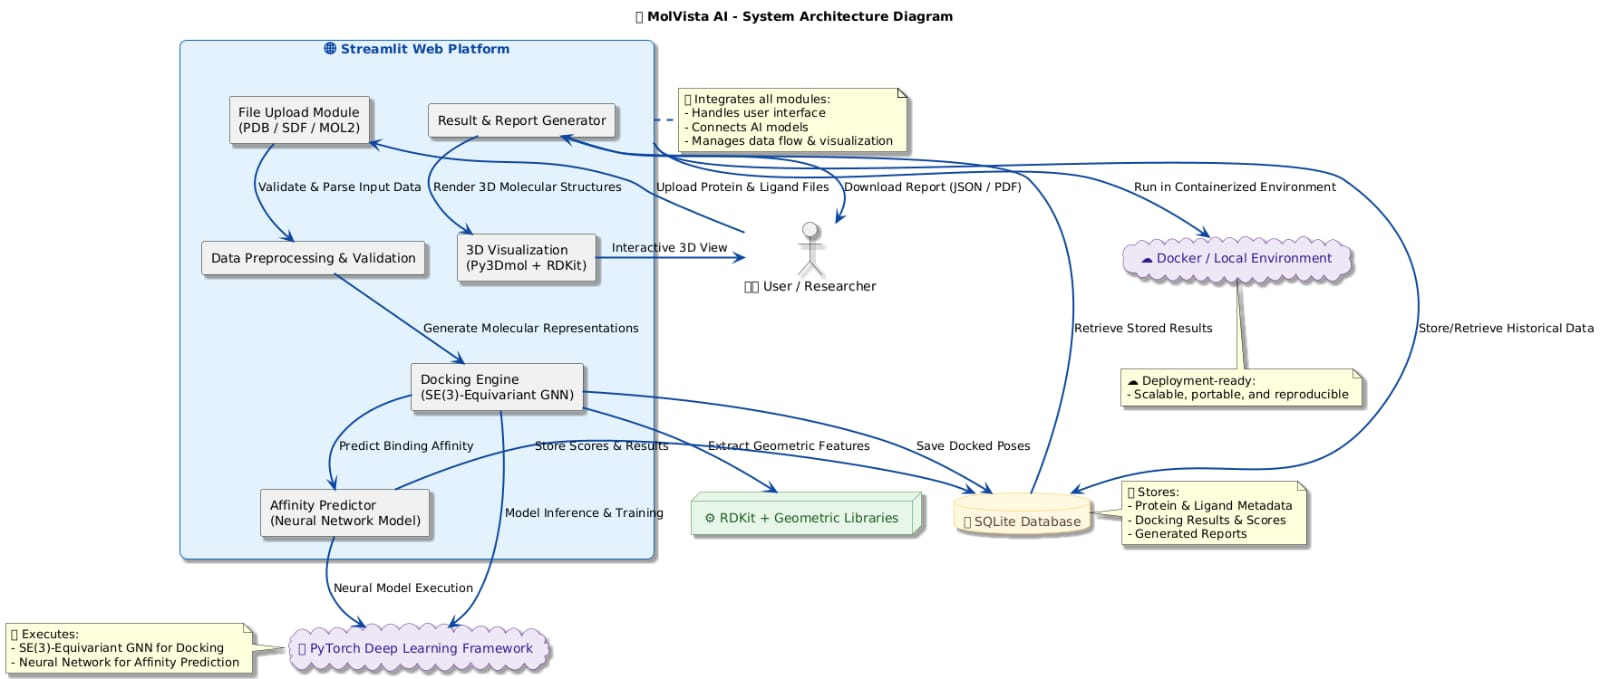
\includegraphics[width=\linewidth, keepaspectratio]{SystemArchitectureDiagram.jpeg}
    \caption{High-Level System Architecture of MolVista AI}
    \label{fig:architecture}
\end{figure}

\hspace*{0.3in}Figure \ref{fig:architecture} illustrates the overall architecture of the \textbf{MolVista AI} platform. The diagram shows how the different modules—including the Streamlit frontend, AI-powered docking engine, deep learning models, and database components—work cohesively. This design ensures smooth data flow from user input to molecular docking prediction, 3D visualization, and output generation.

\section{Overview of Project Modules}

\hspace{0.3in}The MolVista AI platform contains different interlinked modules that perform specialized tasks while maintaining seamless interoperability. Together these modules support molecular generation, docking, binding affinity prediction, optimization, and visualization within an intuitive web environment.

\begin{itemize}
    \item \textbf{Module 1: Molecule Generator}
    
    \hspace{0.3in}Responsible for creating novel chemical compounds using generative deep learning models such as VAEs or GANs. Key processes include:
    \begin{itemize}
        \item Encoding molecular structures into latent spaces for model input
        \item Sampling latent vectors to generate valid, synthesizable molecules
        \item Exporting molecules in SMILES or SDF formats for downstream docking and analysis
    \end{itemize}

    \item \textbf{Module 2: Molecular Docking Engine}
    
    \hspace{0.3in}Performs protein-ligand docking simulations using an AI-assisted approach. Employs SE(3)-equivariant Graph Neural Networks (GNNs) to predict docking poses while preserving 3D rotational and translational symmetry.

    \item \textbf{Module 3: Affinity Prediction Module}
    
    \hspace{0.3in}Estimates the binding strength between ligands and target proteins based on docking results. Steps include:
    \begin{itemize}
        \item Extraction of geometric and chemical descriptors from docked complexes
        \item Feeding features into the SE(3)-equivariant neural model
        \item Outputting quantitative metrics including predicted docking score, QED, and synthetic accessibility (SA) score
    \end{itemize}

    \item \textbf{Module 4: Molecule Optimization Module}
    
    \hspace{0.3in}Enhances molecular properties through reinforcement learning, optimizing for drug-likeness and affinity. Features:
    \begin{itemize}
        \item The RL agent updates molecular structures guided by reward functions
        \item Iteratively improves compounds and returns them to the generator for refinement
        \item Balances bioactivity with synthetic feasibility
    \end{itemize}

    \item \textbf{Module 5: Data Preprocessing and Validation}
    
    \hspace{0.3in}Ensures input and generated data are clean, complete, and formatted correctly. Functions include:
    \begin{itemize}
        \item Parsing PDB, SDF, or MOL2 files and validating structural correctness
        \item Correcting errors and normalizing data for consistent processing
        \item Preparing 3D structures suitable for model inference
    \end{itemize}

    \item \textbf{Module 6: 3D Visualization Module}
    
    \hspace{0.3in}Provides interactive molecular visualization using Py3Dmol and RDKit:
    \begin{itemize}
        \item Enables rotation, zooming, and highlighting of specific atoms or residues
        \item Displays docking poses alongside affinity and optimization metrics
        \item Supports multiple visualization modes such as cartoon, stick, and surface representations
    \end{itemize}

    \item \textbf{Module 7: Results and Report Generator}
    
    \hspace{0.3in}Compiles analysis outputs into structured reports:
    \begin{itemize}
        \item Summarizes docking scores, QED, SA scores, and molecular properties
        \item Exports results in JSON, CSV, or PDF formats
        \item Facilitates one-click download of all generated molecular data and metrics
    \end{itemize}

    \item \textbf{Module 8: Database Management Module}
    
    \hspace{0.3in}Handles storage and retrieval of molecular data and metadata:
    \begin{itemize}
        \item Uses SQLite for ligand and protein metadata, docking outcomes, and generated molecules
        \item Supports quick access to historical runs and results
        \item Ensures data integrity and reproducibility of experiments
    \end{itemize}

    \item \textbf{Module 9: Web Interface and Integration}
    
    \hspace{0.3in}Offers a user-friendly interface built with Streamlit:
    \begin{itemize}
        \item Facilitates file uploads, docking requests, and result visualization
        \item Integrates backend AI modules and manages workflow execution
        \item Supports local deployment through Docker for portability and scalability
    \end{itemize}
\end{itemize}

\hspace{0.3in}All modules are designed to be modular and interoperable, enabling efficient data flow from molecule creation to evaluation and optimization. This architecture accelerates drug discovery while maintaining high prediction accuracy and system robustness.

\section{User Interface}

\hspace{0.3in}The user interface of \textbf{MolVista AI} is created so as to be clear and easy to navigate which provides annotated visual cues and controls allowed to interact with every stage of the workflow. It has an intuitive access to file uploads, docking execution, visualization and result management.

\begin{figure}[H]
    \centering
    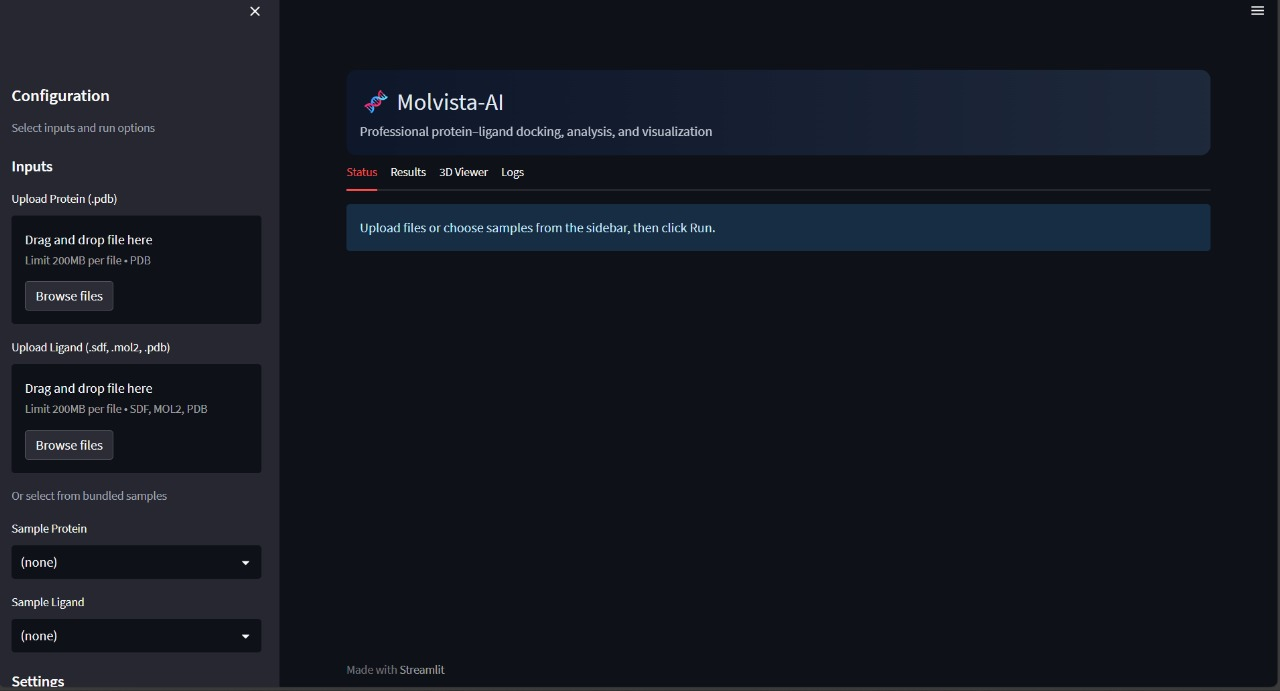
\includegraphics[width=0.95\textwidth]{landing.jpeg}
    \caption{File Upload Interface Landing Page}
\end{figure}

\begin{itemize}
    \item Allows drag and drop based or manual selection of protein and ligand file (.PDB, .SDF, .MOL2).
    \item Shows separate input sections and sample datasets for the convenience of the user.
    \item Is able to validate molecular structures on upload and having immediate feedback.
    \item Has a clean and minimalistic appearance for easy navigation.
\end{itemize}

\begin{figure}[H]
    \centering
    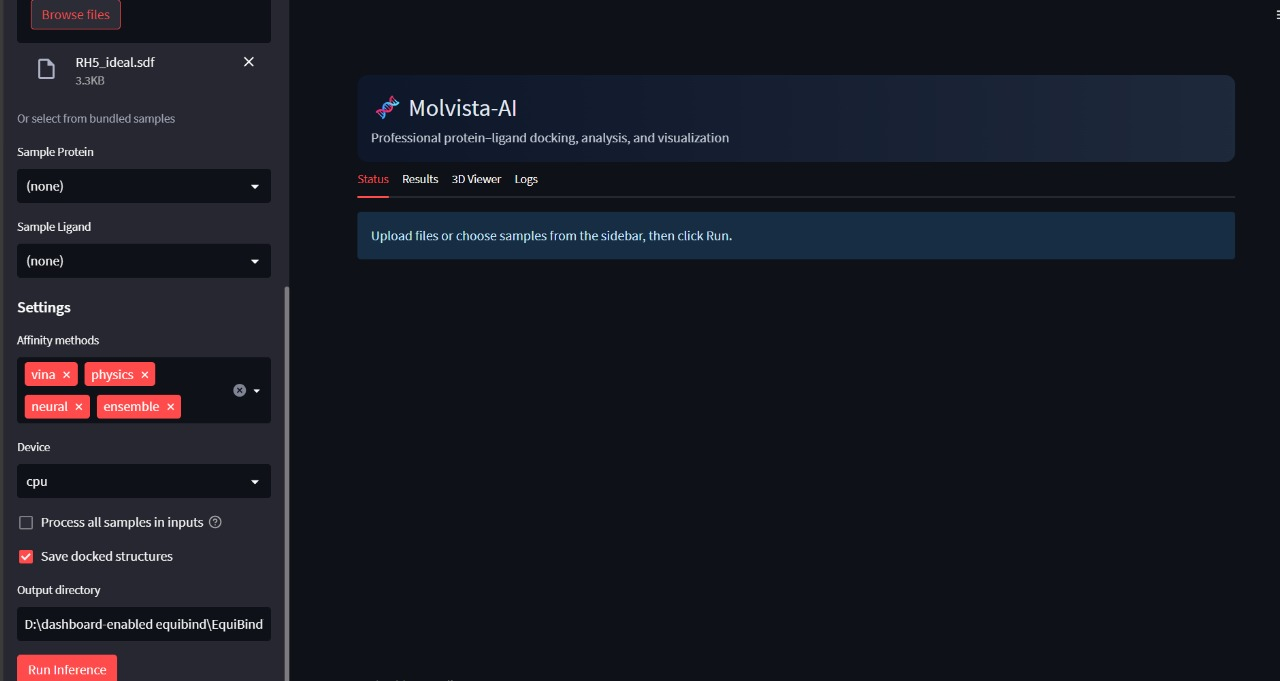
\includegraphics[width=0.95\textwidth]{home.jpeg}
    \caption{Home Screen: Docking Configuration Panel}
\end{figure}

\begin{itemize}
    \item Main dashboard to set docking and affinity prediction dependent parameters.
    \item Affinity calculation methods are offered (Vina, Physics, Neural, Ensemble).
    \item Incidentally CPUs/GPUs can be configured as well as the output directory and batch settings.
    \item Supports saving the properties of docked structures and multi protein-ligand tasks.
\end{itemize}

\begin{figure}[H]
    \centering
    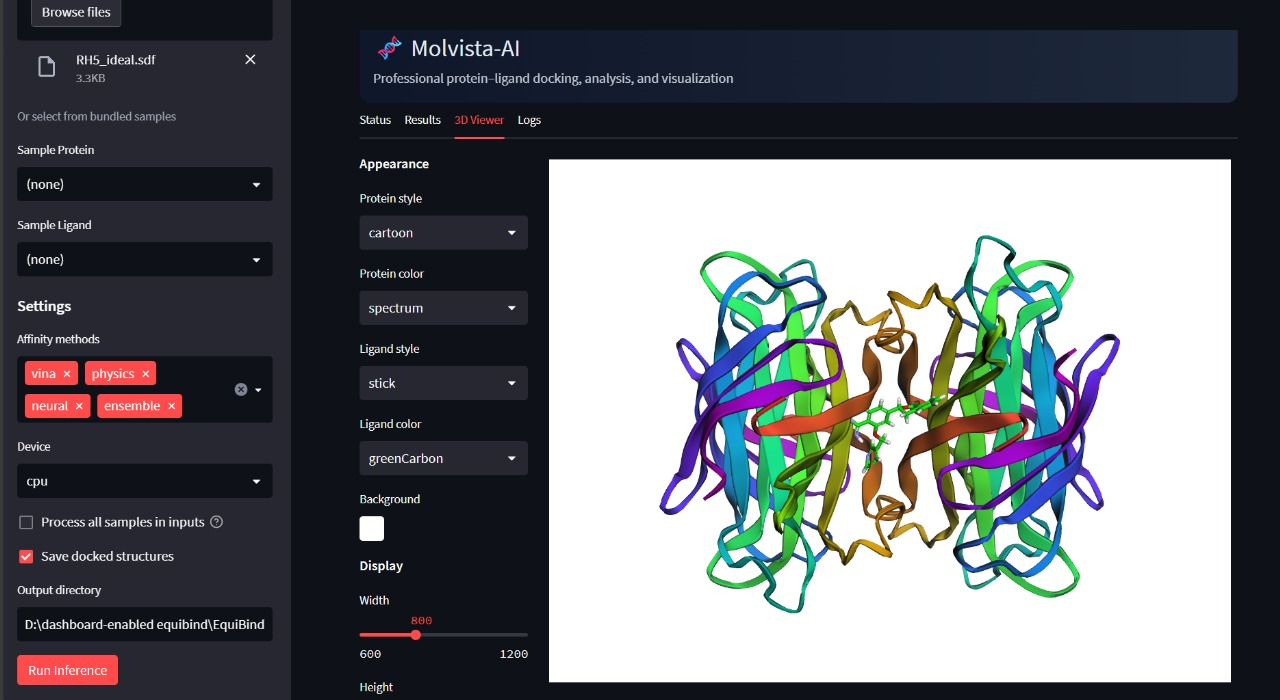
\includegraphics[width=0.95\textwidth]{mol.jpeg}
    \caption{3D Visualization Window}
\end{figure}

\begin{itemize}
    \item Interactive molecular visualization (Py3Dmol).
    \item modes of representations: cartoon, stick, surface.
    \item Fully customize able color schemes and structural styles.
    \item Rotation, zoom and scale in real-time, to provide the detailed structural analysis.
\end{itemize}

\begin{figure}[H]
    \centering
    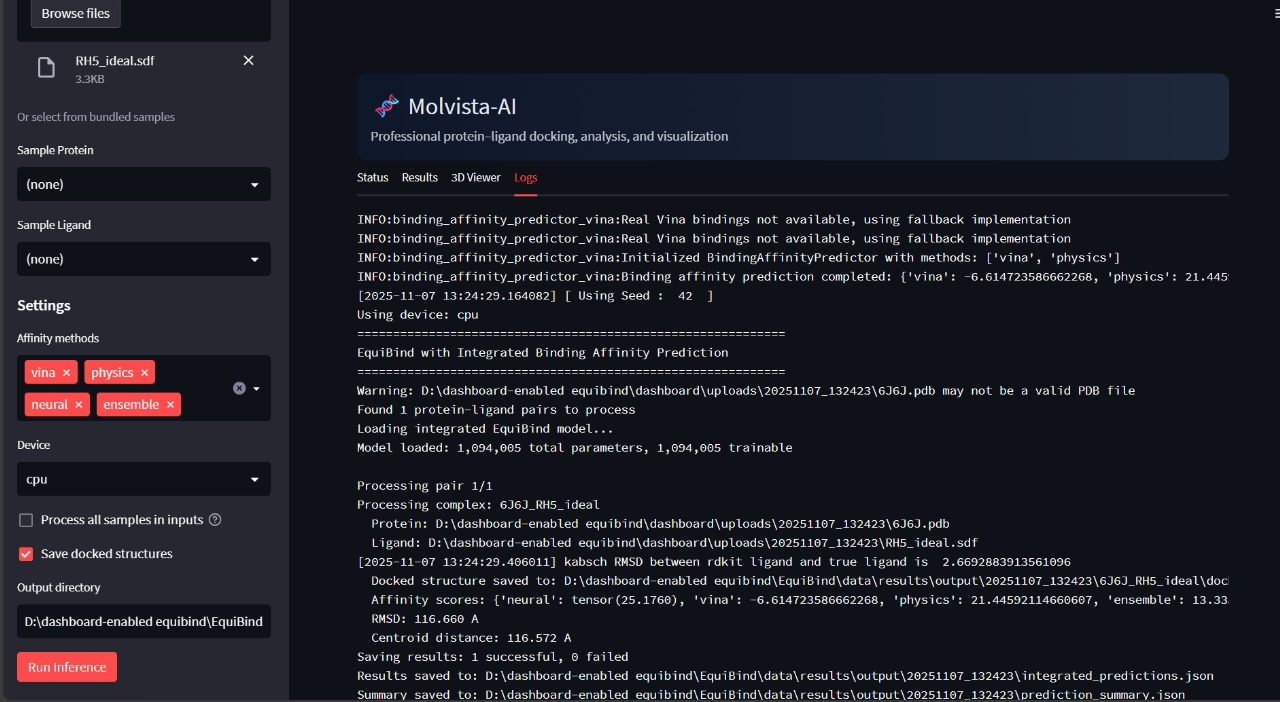
\includegraphics[width=0.95\textwidth]{logs.jpeg}
    \caption{Docking Execution and Log Panel}
\end{figure}

\begin{itemize}
    \item Displays live docking progress with detailed logs of operations of the AI models.
    \item Displaying device allotment, computed steps and center outcome.
    \item Logs the full transparency of all parameters and affinity predictions.
    \item Allows for real-time monitoring of the completion of docking and predictions.
\end{itemize}

\begin{figure}[H]
    \centering
    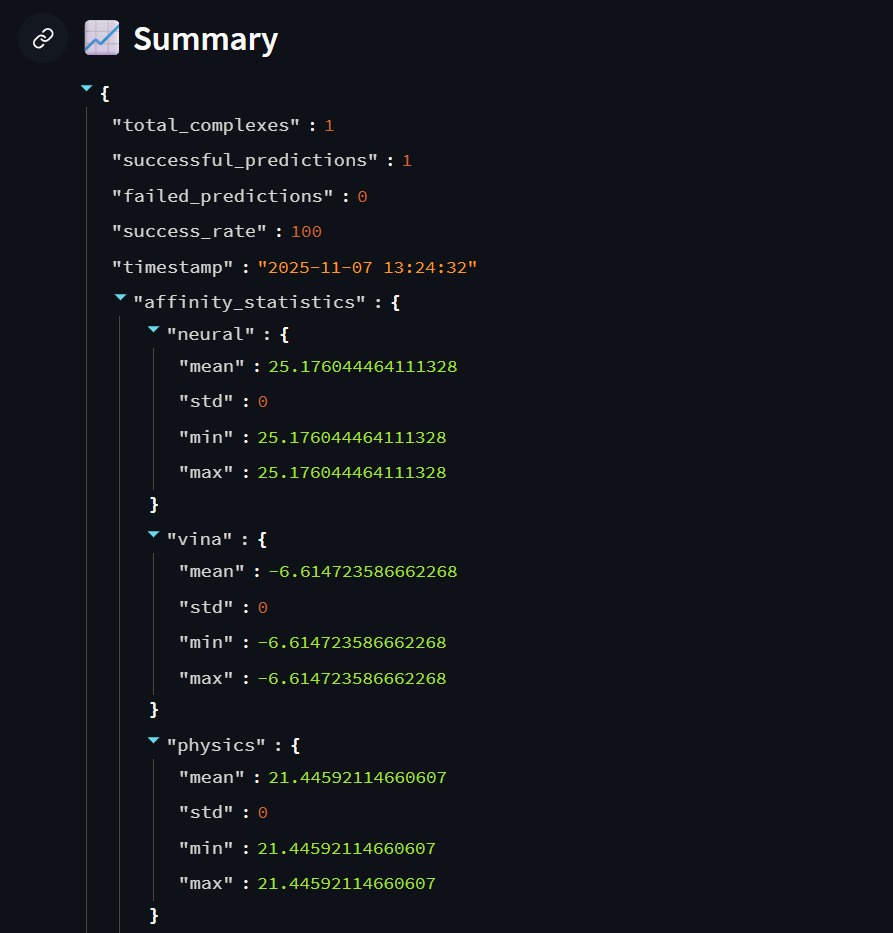
\includegraphics[width=0.75\textwidth]{summ.jpeg}
    \caption{Summary and Results Panel}
\end{figure}

\begin{itemize}
    \item Summarizes processed complexes, docking success rates and performance numbers.
    \item Shows the statistics of affinity such as min, max and mean values between models.
    \item Helps users to compare predictions and validate the docking accuracy
    \item Supports exporting detail reports and all passed data to further analyse.
\end{itemize}

\section{Data Design}

\subsection{Data Structure}
\hspace{0.3in} The \textbf{MolVista AI} system exploits various types of recombination of structured information, semi structured and temporary data structures to support its high efficiency processing of molecular data, the prediction of molecular docking and the ability to afford assessing the affinity in a A.I.-based system. These types of structures are carefully designed to accommodate massive molecular datasets, and ensure modularity, interpretability and scalability amongst all the computational modules.

\vspace{0.4cm}
\begin{enumerate}[label=\textbf{\Alph*.}, leftmargin=1.2cm]
    
    \item \textbf{Internal Data Structures}
    \begin{itemize}
        \item \textbf{Representations of Molecule Graph:}
        \begin{itemize}
            \item Each molecular entity (ligand or protein) is internally modeled as a graph, in which atoms are nodes and the bonds are edges.
            \item Node features such as types (atom type), hybridization and partial charges, adjacency matrices are stored in NumPy and PyTorch tensor format.
            \item These graph structures are the direct input in the SE(3)-equivariant over the network Graph Neural Network (GNN) applied in docking simulations.
        \end{itemize}

        \item \textbf{3D Coordinate Matrices:}
        \begin{itemize}
            \item 3D molecular coordinates are stored in matrix form with respect to the atomic indices.
            \item These are the matrices that enable geometric transformation, such as rotations and translations, so as to provide spatial invariance for the inference.
        \end{itemize}

        \item \textbf{Tensor Data Arrays:}
        \begin{itemize}
            \item Extracted spatial features obtained from molecular complexes stored as PyTorch tensor arrays.
            \item These arrays serve as the go-between between the docking engine and the affinity predictor, which helps reduce serialization cost and increases the GPU processing efficiency.
        \end{itemize}

        \item \textbf{Feature Dictionaries:}
        \begin{itemize}
            \item Key-value dictionaries that may associate molecular IDs with molecular descriptors such as QED (Quantitative Estimate of Drug-likeness), SA (Synthetic Accessibility), as well as the molecular weight
            \item These make it possible to perform fast lookups during optimization and report generation.
        \end{itemize}
    \end{itemize}

    \vspace{0.4cm}
    \item \textbf{Global Data Structures}
    \begin{itemize}
        \item \textbf{Model Weights and Parameters:}
        \begin{itemize}
            \item Global objects for storing trained weights for the SE(3)-Equivariant GNN, Neural Affinity Predictor.
            \item Parameters are transferred to the GPUs memory at run-time in order to save overhead when loading.
        \end{itemize}

        \item \textbf{Configuration / Metadata Objects:}
        \begin{itemize}
            \item Configuration files in the form of JSON files to specify hyperparameters such as learning rate, number of iterations for docking, and checkpoint path of the model.
            \item Metadata, e.g. PDBBind, MOSES, preprocessing pipeline version.
        \end{itemize}

        \item \textbf{Database Tables:}
        \begin{itemize}
            \item SQLite tables, in which structured protein-ligand metadata, docking results, affinity scores and generated molecules will ultimately be stored.
            \item Primary keys guarantee referential integrity and consistent access across all modules that run in the system.
        \end{itemize}
    \end{itemize}

    \vspace{0.4cm}
    \item \textbf{Temporary Data Structures}
    \begin{itemize}
        \item \textbf{Ephemeral Memory Buffers:}
        \begin{itemize}
            \item During real-time docking and affinity computations, intermediate data like energy scores, embeddings and predicted coordinates are stored at buffers in GPU memory.
            \item Buffers are cleared automatically after every iteration so as to maintain memory efficiency.
        \end{itemize}

        \item \textbf{Batch Queues:}
        \begin{itemize}
            \item Dynamic data loaders are bits of batched molecular samples, for temporarily stored purpose to feed efficiently models.
            \item Such queues are used to balance the computation load and for performing asynchronous I/O operations for scalability.
        \end{itemize}

        \item \textbf{Session Logs and Report Caches:}
        \begin{itemize}
            \item Docking logs, predicted affinities and molecular visualization outputs are cached into the web session.
            \item Once data is processed, if the data processing is finished, temporary copies of data are moved to permanent storage or automatically cleared for maintaining same performance.
        \end{itemize}
    \end{itemize}
\end{enumerate}

\subsection{Database Description}

\vspace{0.3cm}
\hspace{0.3in} The \textbf{MolVista AI} database is designed for effective molecular data management, maintaining integrity, reproducibility, and scalability in AI aiding in docking and affinity prediction workflows. It builds upon information concerning proteins, ligands and docking outcomes through relation tables and is compatible with user-driven or automatic processes. The schema of the database is lightweight, modular and is optimized for high-speed query respondence in real-time analytics.

\vspace{0.4cm}
\begin{itemize}
\vspace{0.3cm}
\item \textbf{User:}
\begin{itemize}
\item Stores information about researchers and users of the platforms
\item Attributes (user\_id, name, email, and organization).
\item Parent entity linking uploaded proteins and ligands using foreign keys.
\end{itemize}

\item \textbf{Protein:}
\begin{itemize}
\item Contains uploaded structures of proteins in PDB file format that has 3D coordinates and metadata attribute.
\item Fields: protein\_id, user\_id (FK), name, pdb\_file, upload\_date
\item each protein is linked to its uploader and can be involved in more than one docking experiment.
\end{itemize}

\item \textbf{Ligand:}
\begin{itemize}
\item Includes uploaded ligand file in SDF or MOL2 Format
\item Attributes of table are \texttt{ligand\_id}, \texttt{user\_id (FK)}, \texttt{name}, \texttt{sdf\_file} and \texttt{upload\_date}.
\item Ligands corresponds to their uploader and can be associated with several proteins.
\end{itemize}

\item \textbf{DockingResult:}
\begin{itemize}
\item Contains results from the docking engine.
\item Attributes: \texttt{result\_id}, \texttt{protein\_id (FK)}, \texttt{ligand\_id (FK)}, \texttt{affinity\_score}, \texttt{rmsd}, \texttt{pose\_file}, \texttt{date\_generated}
\item Affinity score is an indicator of predicted binding strength; RMSD is an indicator of accuracy of the docking pose.
\item Pose files are stored for the 3D visualizations and for AI model training.
\end{itemize}

\item \textbf{Report:}
\begin{itemize}
\item Stores final reports and processed outputs of each docking run.
\item Attributes: \texttt{report\_id}, \texttt{result\_id (FK)}, \texttt{json\_file}, \texttt{pdf\_file}, \texttt{generated\_on}.
\item Reports: Consists of gathering docking results, interaction maps and predicted affinities (in the formats of JSON and PDF).
\end{itemize}
\end{itemize}

\vspace{0.4cm}
\hspace{0.3in} This referential integrity is enforced through the use of foreign key constraints that connect the docking results and reports to its respective proteins, ligands, and users. This structure delivers optimal query performance, provides seamless integration of AI pipelines and guarantees reproducible and scalable molecular data management.

\vspace{0.2cm}
\section{UML Diagrams}
\vspace{0.1cm}
\hspace{0.3in}The UML diagrams are used to give pictorial representations of the structure and behaviors of the \textbf{MolVista AI} system. They show relationships between modules, AI models and user interfaces demonstrating workflows and interactions required for the efficient docking and affinity prediction. Included diagrams for use cases, sequences, classes, activities, as well as deployment, which will collectively show how the platform will achieve modular, transparent, and high-performance, molecular analysis.

\begin{itemize}
\item \textbf{Use Case Diagram} \\
\hspace{0.3in}The use case diagram is used to identify prominent actors such as researchers and administrators, and main functionalities like uploading files, docking, predicting affinities, visualization, generating reports, etc. This visualization helps to clarify the functional boundaries in the system and illustrate the way that the users interact with various modules during the execution of the molecular analysis workflow.

\begin{figure}[H]
\centering
% Maintain rotation 0 for a portrait alignment
\rotatebox{0}{%
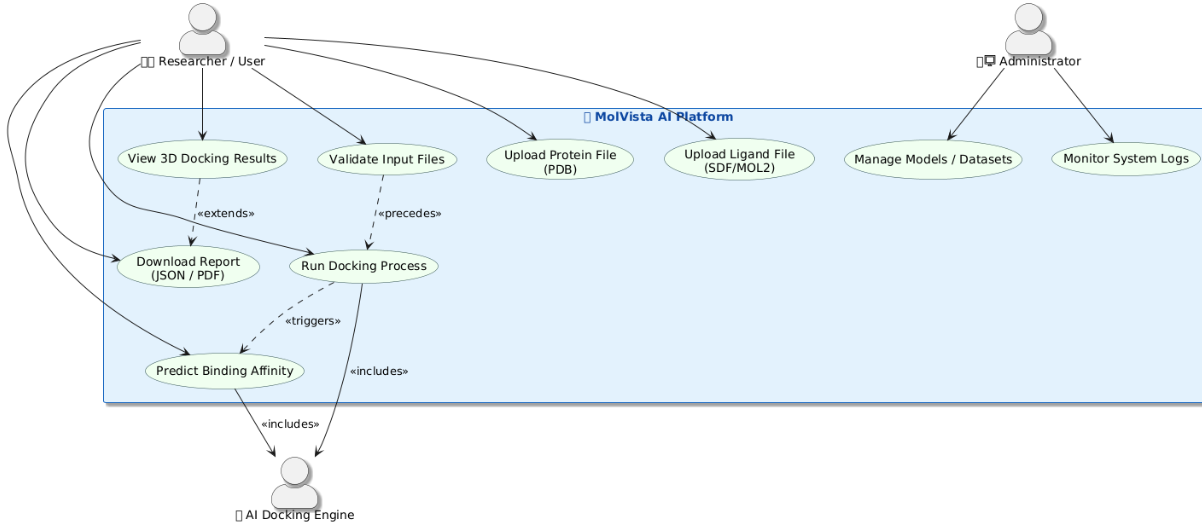
\includegraphics[width=16cm, height=10cm]{./UseCase.png}%
}
\caption{Use Case Diagram}
\label{fig:usecase}
\end{figure}

\vspace{0.8cm}

\item \textbf{Use Case Scenarios} \\
\hspace{0.3in}The use case scenarios offer a structured tabular view of every functional element in the context of MOLVista AI. Each scenario specifies the purpose of the scenario, the actors involved, the input and output flow, the preconditions and exception handling. This structured documentation allows for a detailed understanding of the interactions and interactions between modules of the system, for example file uploads, docking execution, affinity prediction and visualization, to achieve the overall functional objectives of the platform.

\renewcommand{\arraystretch}{1.3}

\begin{longtable}{|p{3.5cm}|p{10.5cm}|}
\caption{Use Case Summary} \\ \hline
\textbf{System Name} & MolVista AI Platform \\ \hline
\textbf{Primary Actors} & Researcher/User, Administrator \\ \hline
\textbf{Supporting Actors} & AI Docking Engine \\ \hline
\textbf{Goal} & To do AI-based Protein-ligand docking, predict the affinity to bind \& be able to visualize molecular bonding and efficient management of models and data sets. \\ \hline
\end{longtable}

%--------------------------- Use Case 1 ----------------------------
\begin{longtable}{|p{4cm}|p{9.8cm}|}
\caption{Use Case 1 - Upload Protein File (PDB)} \\ \hline
\textbf{Actor} & Researcher/ User \\ \hline
\textbf{Description} & The user uploads a protein structure file in PDB format file to create a new docked protein that would start the docking procedure. \\ \hline
\textbf{Precondition} & The user is authenticated \& The user has access to the upload interface. \\ \hline
\textbf{Postcondition} & Protein file is stored and validated (correct structure) successfully. \\ \hline
\textbf{Includes} & Validate Input Files \\ \hline
\textbf{Triggers} & User clicks "Upload Protein File" option. \\ \hline
\textbf{Exceptions} & Invalid format OR corrupted file OR unsupported PDB structure. \\ \hline
\end{longtable}

%--------------------------- Use Case 2 ----------------------------
\begin{longtable}{|p{4cm}|p{9.8cm}|}
\caption{Use Case 2-Upload Ligand File(SDF/MOL 2)} \\ \hline
\textbf{Actor} & Researcher/ User \\ \hline
\textbf{Description} & User Uploads ligand file in SDF or MOL2 Format for Binding Simulation. \\ \hline
\textbf{Precondition} & Protein file must be uploaded and validated. \\ \hline
\textbf{Postcondition} & The ligand file is validated and readied for docking. \\ \hline
\textbf{Includes} & Validate Input Files \\ \hline
\textbf{Triggers} & User clicks on "Upload Ligand File" option. \\ \hline
\textbf{Exceptions} & Unsupported format, no atom data, or upload halted. \\ \hline
\end{longtable}

%--------------------------- Use Case 3 ----------------------------
\begin{longtable}{|p{4cm}|p{9.8cm}|}
\caption{Use Case 3 - Validate Input Files} \\ \hline
\textbf{Actor} & AI Docking Engine \\ \hline
\textbf{Description} & Validates both uploaded files in case of compatibility and completion of data and starts the docking. \\ \hline
\textbf{Precondition} & Protein and ligand files have been successfully uploaded. \\ \hline
\textbf{Postcondition} & Valid inputs are sent to the docking engine. \\ \hline
\textbf{Includes} & -- \\ \hline
\textbf{Triggers} & Completion of file uploads. \\ \hline
\textbf{Exceptions} & File validation fails due to missing or invalid data. \\ \hline
\end{longtable}

%--------------------------- Use Case 4 ----------------------------
\begin{longtable}{|p{4cm}|p{9.8cm}|}
\caption{Use Case: Run Docking Process} \\ \hline
\textbf{Actor} & AI Docking Engine \\ \hline
\textbf{Description} & Enacts the docking process using algorithms that are trained with AI to predict predicted binding poses and elements. \\ \hline
\textbf{Precondition} & Protein and ligand files are supplied, which are valid. \\ \hline
\textbf{Postcondition} & Docking results and interaction models are generated. \\ \hline
\textbf{Includes} & Predict Binding Affinity \\ \hline
\textbf{Triggers} & User clicks "Run Docking Process" \\ \hline
\textbf{Exceptions} & Model execution error, lack of computational resources, or timeout. \\ \hline
\end{longtable}

%--------------------------- Use Case 5 ----------------------------
\begin{longtable}{|p{4cm}|p{9.8cm}|}
\caption{Use Case 5 - Predict Binding Affinity} \\ \hline
\textbf{Actor} & AI Docking Engine \\ \hline
\textbf{Description} & Estimates the binding strength \& Estimates the binding strength and stability of a protein-ligand complex using both neural \& physics-based models. \\ \hline
\textbf{Precondition} & Docking process successfully completed. \\ \hline
\textbf{Postcondition} & Binding Affinity results created store in the database. \\ \hline
\textbf{Includes} & -- \\ \hline
\textbf{Triggers} & Completion of docking execution. \\ \hline
\textbf{Exceptions} & Missing Parameters or Model Inference failed. \\ \hline
\end{longtable}

%--------------------------- Use Case 6 ----------------------------
\begin{longtable}{|p{4cm}|p{9.8cm}|}
\caption{Use Case 6 - View 3D Docking Results} \\ \hline
\textbf{Actor} & Researcher/ User \\ \hline
\textbf{Description} & Shows 3d molecular visualization results from protein-ligand docking active in an interactive viewer. \\ \hline
\textbf{Precondition} & Output data of a docking is available. \\ \hline
\textbf{Postcondition} & Visualization Were loaded with modification options for viewing. \\ \hline
\textbf{Triggers} & User selects "View 3D Docking Results". \\ \hline
\textbf{Exceptions} & Browser rendering error, issue compatibility GPU. \\ \hline
\end{longtable}

%--------------------------- Use Case 7 ----------------------------
\begin{longtable}{|p{4cm}|p{9.8cm}|}
\caption{Use Case 7 - Download Report (JSON / PDF)} \\ \hline
\textbf{Actor} & Researcher/ User \\ \hline
\textbf{Description} & Retrieves data from the docking to export the summary of the docking and the affinity predictions in the form of a survey of the results in the form of a report (in pdf or json). \\ \hline
\textbf{Precondition} & Docking and prediction tasks completed. \\ \hline
\textbf{Postcondition} & Report got generated \& Report downloaded successfully. \\ \hline
\textbf{Triggers} & User clicks "Download Report" button \\ \hline
\textbf{Exceptions} & Failure in report generation, interrupted download. \\ \hline
\end{longtable}

%--------------------------- Use Case 8 ----------------------------
\begin{longtable}{|p{4cm}|p{9.8cm}|}
\caption{Use Case 8 - Managing Models / Datasets} \\ \hline
\textbf{Actor} & Administrator \\ \hline
\textbf{Description} & Enables administrators to update, re-train or configure AI models and datasets to provide optimal performance. \\ \hline
\textbf{Precondition} & Admin privileges checked. \\ \hline
\textbf{Postcondition} & Modified configurations implemented in the system. \\ \hline
\textbf{Triggers} & Admin selects "Manage Models/Datasets" \\ \hline
\textbf{Exceptions} & Unauthorized access, model corruption. \\ \hline
\end{longtable}

\vspace{0.6cm}
\item \textbf{Class Diagram} \\
\hspace{0.3in}The class diagram gives an initial overview on the structural design of the \textbf{MolVista AI} system. It orchestrates such important entities as proteins, ligands, the docking engine, visualization components, and report generators. This is a diagram to understand how the classes interact through associations and inheritance these are like blueprints to help manage data and how to work out computational workflows and how to coordinate module:
\begin{figure}[H]
    \centering
    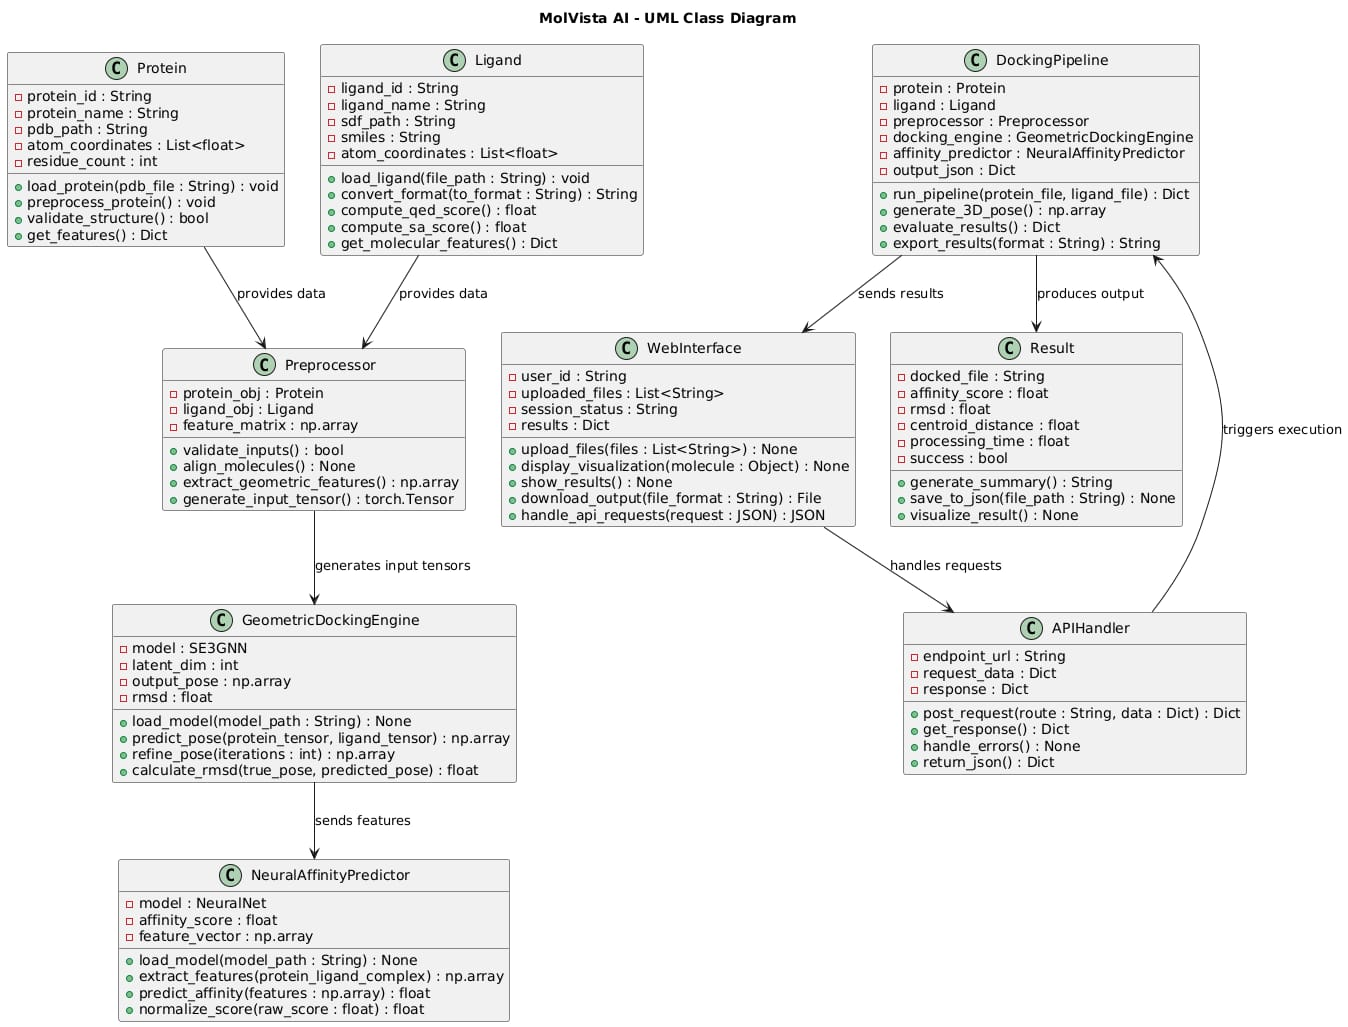
\includegraphics[height=12cm,width=0.9\textwidth]{class.jpeg}
    \caption{Class Diagram}
\end{figure}

\vspace{0.6cm}
\item \textbf{Object Diagram} \\
\hspace{0.3in}The object diagram represents live real instances of the classes of the system at a given point in time. It shows the interaction between objects, such as protein and ligand file, docking results, and visualization components, during the execution process. This diagram gives a way to understand the data flow at runtime and provides a way to check the object level relationships which were defined in a class diagram.
\begin{figure}[H]
    \centering
    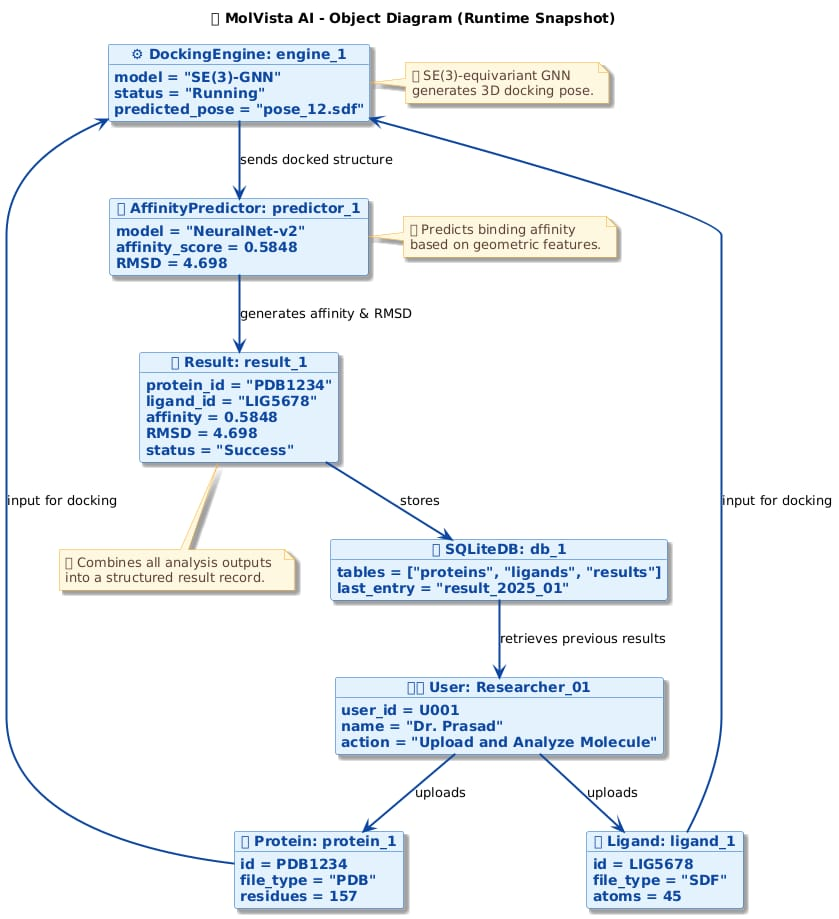
\includegraphics[width=0.9\textwidth]{obj.jpeg}
    \caption{Object Diagram}
\end{figure}

\vspace{0.6cm}
\item \textbf{Sequence Diagram} \\
\hspace{0.3in}The sequence diagram records the time-based interaction between the components of the system in chronological order. It displays the exchange of messages in processes that include file uploads, docking computation, affinity prediction, and 3D visualization. This representation is useful for the analysis of timing, order of execution and dependencies between modules.
\begin{figure}[H]
    \centering
    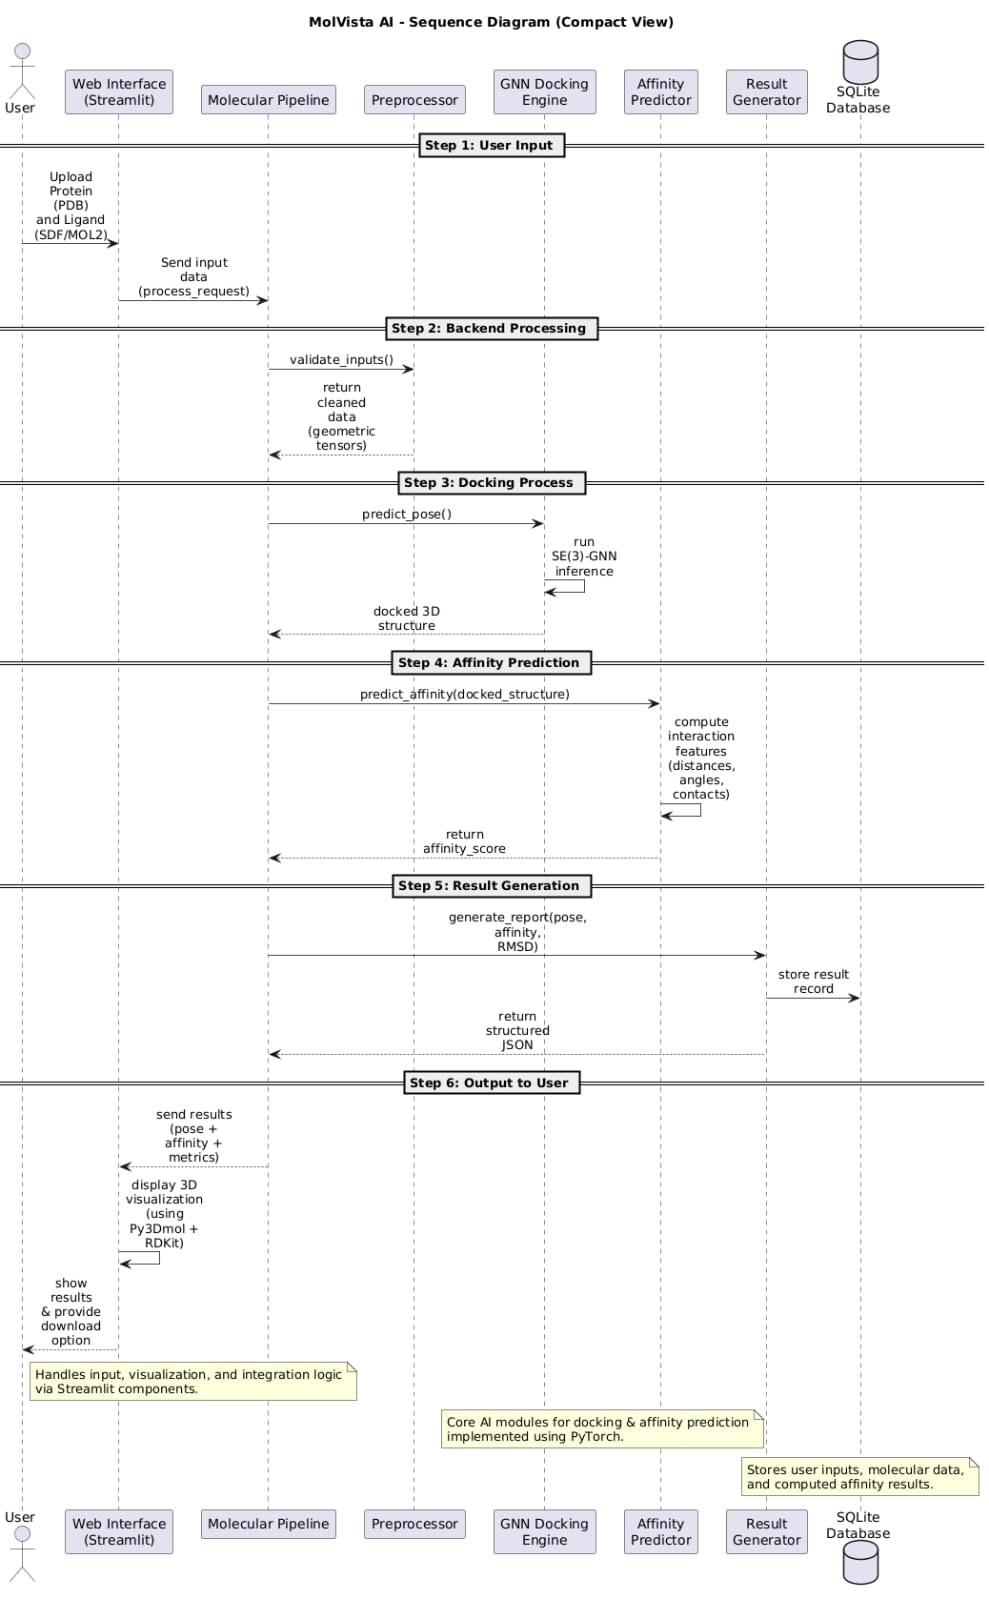
\includegraphics[height=17cm,width=0.9\textwidth]{seq.jpeg}
    \caption{Sequence Diagram}
\end{figure}

\item \textbf{Activity Diagram} \\
\hspace{0.3in}The activity diagram describes the full work leading process of the system including the order of operations and decision points between input and output. It shows transitions from one step to another e.g. validation, processing, and visualization to provide a clear picture of the logical flow of the operations.
\begin{figure}[H]
    \centering
    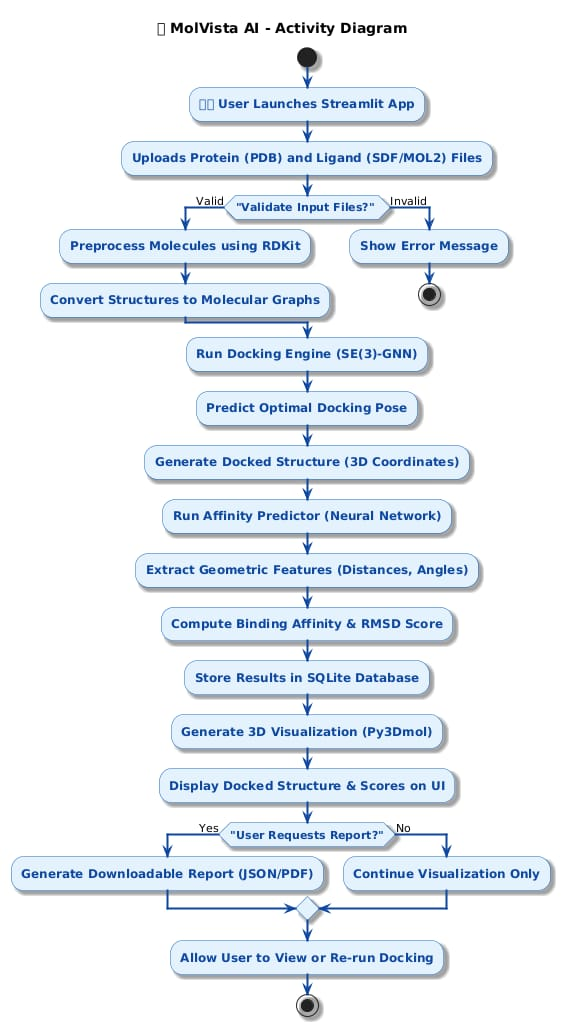
\includegraphics[height=17cm,width=0.9\textwidth]{ActivityDiagram.jpeg}
    \caption{Activity Diagram}
\end{figure}

\item \textbf{Component Diagram} \\
\hspace{0.3in}The component diagram plays the role of presenting the modular structure of \textbf{MolVista AI} that consist of dividing the system into distinct functional units. It represents the interactions between components, sometimes the user interface, sometimes the docking engine, sometimes the artificial intelligence modules, sometimes the report generator, and provides emphasis on maintainability, modularity and scalability.
\begin{figure}[H]
    \centering
    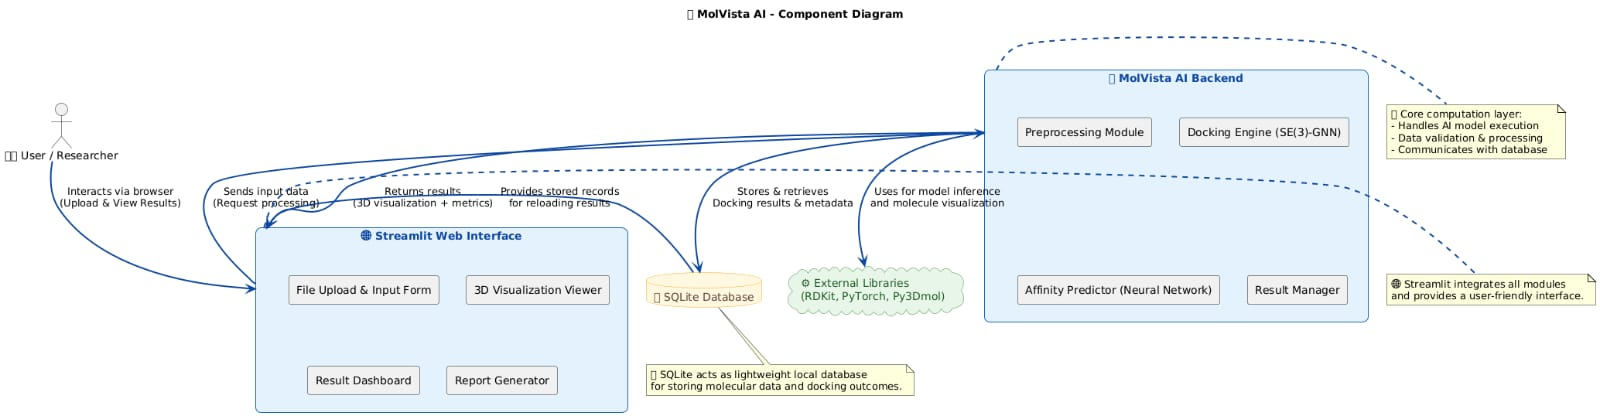
\includegraphics[height=6cm,width=0.9\textwidth]{comp.jpeg}
    \caption{Component Diagram}
\end{figure}

\vspace{0.6cm}
\item \textbf{Data Flow Diagram (Level 0)} \\
\hspace{0.3in}The Level 0 DFD provides an overview of the system at the top level to describe the major data flows between the external entities and the basic processes. It connects to a general workflow - it points out important inputs, outputs, and storage spots.
\begin{figure}[H]
    \centering
    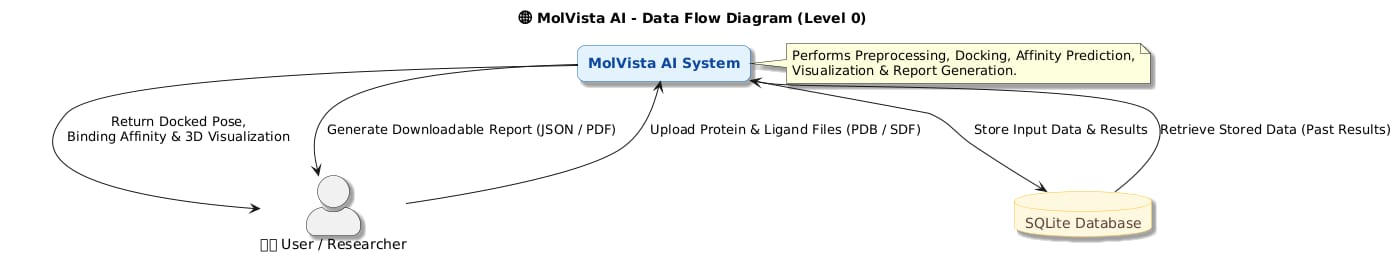
\includegraphics[height=6cm,width=0.9\textwidth]{dfd0.jpeg}
    \caption{Data Flow Diagram - Level 0}
\end{figure}

\vspace{0.6cm}
\item \textbf{Data Flow Diagram (Level 1)} \\
\hspace{0.3in}The Level 1 DFD is used to expand the main system process into more sub-processes. It tracks the movement of data between modules like validation, artificial intelligence computation and result generation, to enable detailed view of the module dependencies and transformations.
\begin{figure}[H]
    \centering
    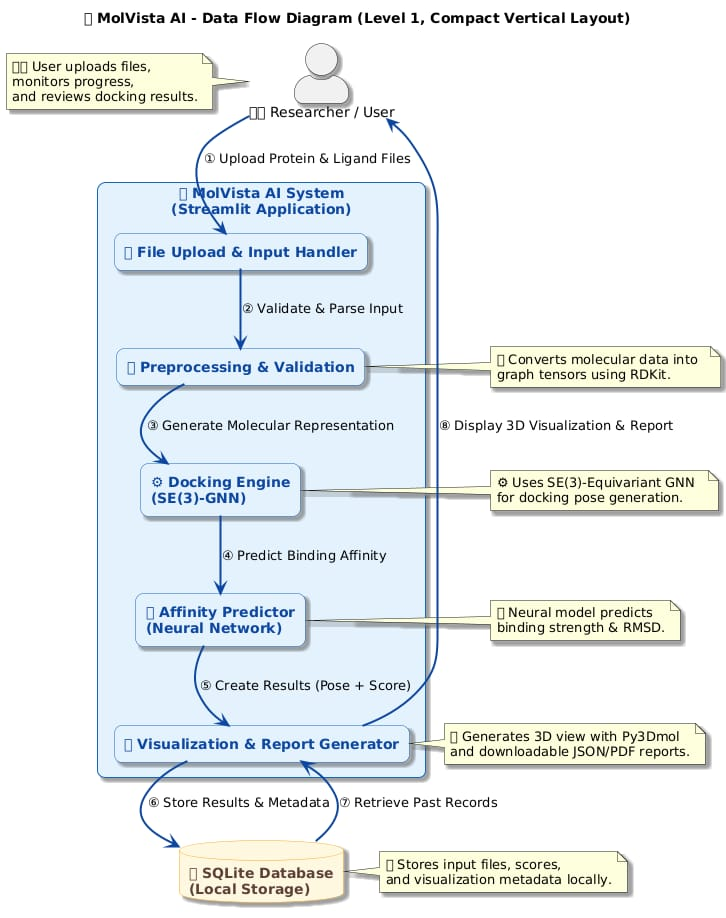
\includegraphics[height=17cm,width=0.9\textwidth]{dfd1.jpeg}
    \caption{Data Flow Diagram - Level 1}
\end{figure}

\vspace{0.8cm}
\item \textbf{Data Flow Diagram (Level 2)} \\
\hspace{0.3in}The Level 2 DFD is a granular view of the interactions of the sub-process and routing of data between modules. This is oriented toward information flows through input storage and computational elements to visualization systems with a detailed view inside communications.
\begin{figure}[H]
    \centering
    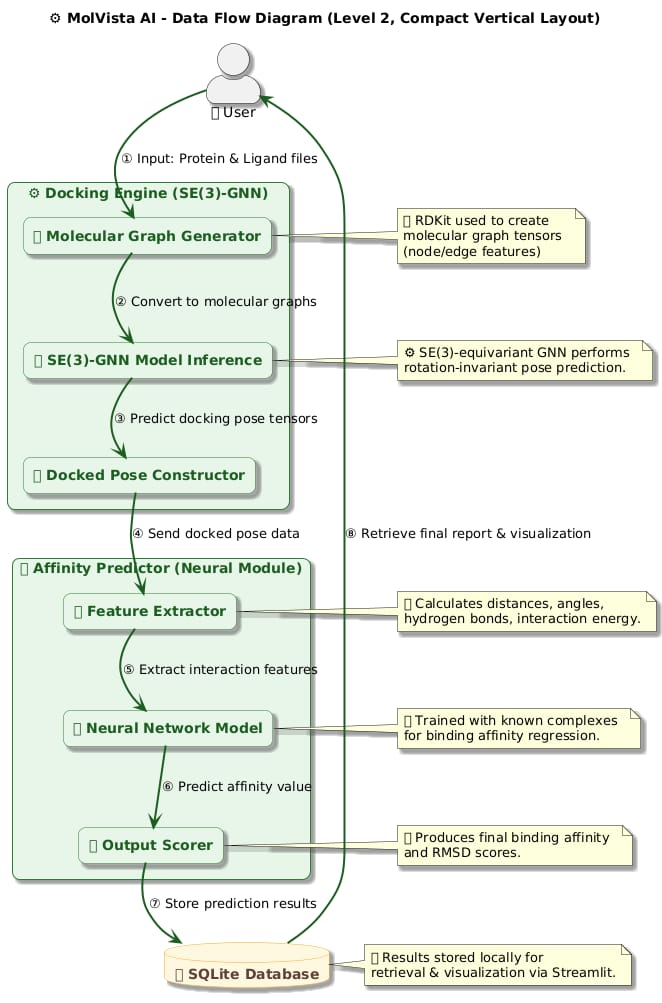
\includegraphics[height=17cm,width=0.9\textwidth]{dfd2.jpeg}
    \caption{Data Flow Diagram - Level 2}
\end{figure}

\item \textbf{Deployment Diagram} \\
\hspace{0.3in}The deployment diagram gives the software components distribution on hardware. It indicates the relationships between the front-end interface, computational modules and the database to ensure efficient use of resources and security in communication across the entire system.
\begin{figure}[H]
    \centering
    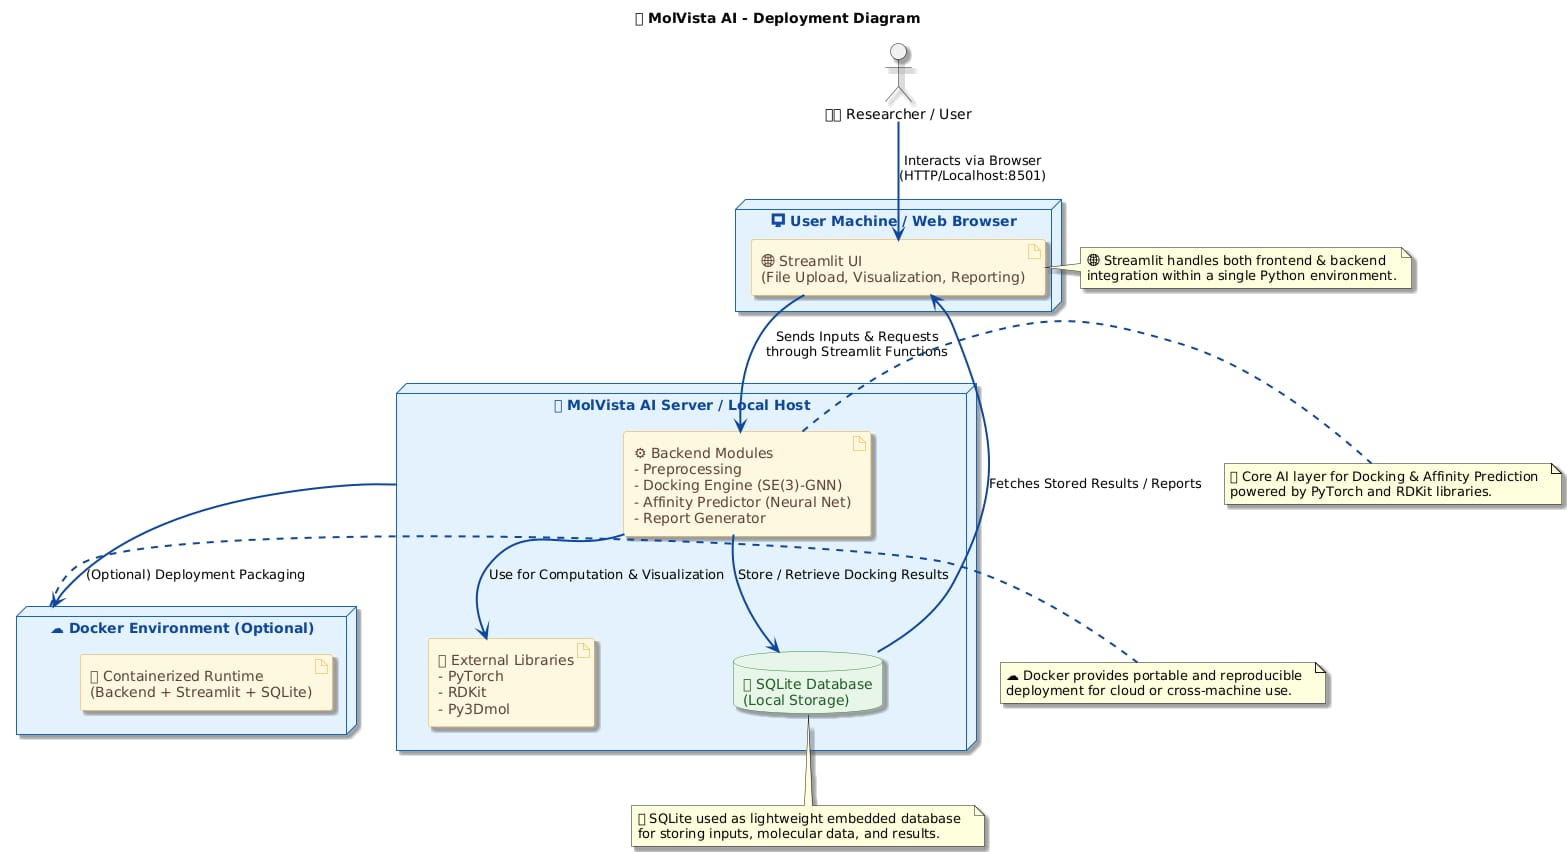
\includegraphics[width=0.9\textwidth]{deploy.jpeg}
    \caption{Deployment Diagram}
\end{figure}
\end{itemize}
\section{Tools and Technology Used}

\begin{itemize}
\item \textbf{Tools}
\begin{enumerate}
\item \textbf{Development Tools}

\noindent \textbf{Programming Languages}
\begin{itemize}
    \item \textbf{Python (FastAPI + PyTorch):} Takes the care of backend services, model training and docking/affinity predictions.
    \item \textbf{JavaScript (Streamlit + React.js):} Handles frontend functionality and 3D molecular visualization.
\end{itemize}

\noindent \textbf{Database}
\begin{itemize}
    \item \textbf{SQLite:} Relational database containing the users, the molecules and docking results and reports.
    \item \textbf{RDKit Integration:} For preprocessing molecules, generating descriptors and validating structures.
\end{itemize}

\noindent \textbf{Version Control And Collaboration}
\begin{itemize}
    \item \textbf{GitHub:} Version controlled repository of backend, artificial intelligence and web modules.
    \item \textbf{Docker:} Containerization for consistent deployment - to local and to the cloud.
\end{itemize}

\vspace{0.3cm}
\item \textbf{Artificial Intelligence and Computational Tools}

\begin{itemize}
    \item \textbf{PyTorch:} Implements SE(3)-Equivariant GNNs and Neural Affinity Predictors.
    \item \textbf{NumPy and SciPy:} Supports matrix operations, numerical operations and energy operations.
    \item \textbf{RDKit:} Parses molecular formats; computes 3D molecular descriptors; produces input data.
    \item \textbf{Py3Dmol:} Provides interactive 3D visualizations within the platform.
\end{itemize}

\vspace{0.3cm}
\item \textbf{Deployment \& Environment Tools}

\begin{itemize}
    \item \textbf{Docker and Kubernetes:} Support for scalable containerized GPUs deployments.
    \item \textbf{Streamlit:} Helps in the quick deployment of interactive AI web applications.
    \item \textbf{Linux (Ubuntu):} Development \& runtime environment for backend \& AI Models.
\end{itemize}

\vspace{0.3cm}
\item \textbf{Visualization and Documentation Tools}

\begin{itemize}
    \item \textbf{Py3Dmol:} Produces interactive 3D views of docked molecules.
    \item \textbf{Matplotlib / Plotly:} Plots affinity scores, RMSD and performance metrics.
    \item \textbf{LaTeX:} Formats reports and technical documentation, and publication-prepared materials.
\end{itemize}

\end{enumerate}

\vspace{0.5cm}
\item \textbf{Techniques}
\begin{enumerate}

\item \textbf{Machine Learning Techniques}
\begin{itemize}
    \item SE(3)-Equivariant Graph Neural Networks for spatially consistent Molecular Representation.
    \item Regression models for predicting ligand-protein binding affinity from data sets such as PDBBind.
    \item Conformational optimization and refinement by docking through reinforcement learning.
\end{itemize}

\vspace{0.3cm}
\item \textbf{Computational Chemistry Techniques}
\begin{itemize}
    \item Extraction geometric feature such as bond distances, angles and hydrogen bonding.
    \item Approximation of Binding energies with learned scoring functions.
    \item Molecular preprocessing from RDKit, to obtain the right 3D structure.
\end{itemize}

\vspace{0.3cm}
\item \textbf{Database and System Techniques}
\begin{itemize}
    \item Normalized relational schema for linking users, molecules, docking results and reports.
    \item Efficient indexing, caching retrieval and comparisons.
    \item JSON reporting and REST API endpoints for structured data sharing and integration.
\end{itemize}

\vspace{0.3cm}
\item \textbf{Deployment and Integration Techniques}
\begin{itemize}
    \item Docker containerization for reproducible GPU enabled deduction.
    \item Parallel processing to deal with several docking tasks at the same time.
    \item Continuous integration using GitHub Actions for automated building and testing.
\end{itemize}

\end{enumerate}
\end{itemize}

\section{Algorithm}
\noindent\textbf{\large $\bullet$ SE(3)-Equivariant Graph Neural Network for Molecular Docking}\\\\
\hspace{0.3in}
The \textbf{MolVista AI} platform is based on an SE(3)-Equivariant Graph Neural Network (GNN) platform which is used to predict protein-ligand interactions. This network is designed to be receptive to three-dimensional rotational and translational symmetries so that predictions are the same no matter the orientation of the molecules. By taking these symmetries into account, the algorithm makes the computations that are not needed, but efficiently optimizes the accuracy of the docking.

\vspace{0.3cm}
\noindent\textbf{\large $\bullet$ Working}
\begin{itemize}
    \renewcommand\labelitemi{--}
    \item \textbf{Graph Based Molecular Encoding:}\\
    \hspace{0.3in}
    Proteins and ligands are denoted as atomic graphs. Nodes are atoms and have such features as atomic number, hybridization state, and partial charge. Edges represent either chemical bonds or proximity in space and have annotations for both type of bonds and distance between atoms.

    \item \textbf{Equivariant Message Passing:}\\
    \hspace{0.3in}
    Atomic features are updated by the passage of messages across edges without distorting 3D geometric relationships. This is to ensure that atomic interactions are constant in any orientation of the molecule.

    \item \textbf{Binding energy prediction: }\\
    \hspace{0.3in}
    After several layers of message-passing proteins and ligands embeddings are concatenated and fed through a regression model to learn the binding affinity and docking score that gives a quantitative relationship for the strength of the interaction.

    \item \textbf{Docking Pose Selection:}\\
    \hspace{0.3in}
    Multiple docking conformations are generated which are then evaluated according to predicted affinity and structural stability and the first ranking pose stored with associated metadata for visualization and for further analysis.
\end{itemize}

\vspace{0.3cm}
\noindent\textbf{\large $\bullet$ Algorithm (Stepwise)}
\begin{enumerate}
    \item \textbf{Input Representation:}
    \begin{itemize}
        \item Load the 3D structures of protein and ligand molecules (PDB/SDF formats).
        \item Convert these into the graphs: Gp = (Vp,Ep) and Gl = (Vl, El)
        \item Feature assignment to nodes and edges:
        \[
        x_i = [Z_i, q_i, h_i], \quad e_{ij} = [d_{ij}, t_{ij}]
        \]
        Where Z_i, is the atomic number, q_i, is the partial charge, d_ij, is the interatomic distance and t_ij, is the type of bond.
    \end{itemize}

    \item \textbf{Feature Embedding:}
    \hspace{0.3in}
    Map atomic features to initial set of embeddings \( h_i^{(0)} \) using learnable linear transformation.

    \item \textbf{Equivariant Message Passing: }
    \begin{itemize}
        \item At each node, aggregate messages from the neighbors:
        \[
        m_i^{(l)} = \sum_{j \in N(i)} \phi_m(h_i^{(l)}, h_j^{(l)}, e_{ij}, r_{ij})
        \]
        \item Update node embeddings using equivariant transformations:
        \[
        h_i^{(l+1)} = \phi_h(h_i^{(l)}, m_i^{(l)})
        \]
        where \( r_{ij}\) is the 3D relative position vector of atoms \( i \) and \( j \), again to maintain rotational consistency is
    \end{itemize}

    \item \textbf{Protein-Ligand Interaction Layer:}
    \hspace{0.3in}
    Encode cross-graph interactions in order for the network to focus on spatial relationship between ligand atoms and protein binding site residues,

    \item \textbf{Affinity Prediction:}
    \hspace{0.3in}
    Pool of protein and ligand embeddings concatenation and then regression head:
    \[
    y_{pred} = \phi_{affinity}(h_p \oplus h_l)
    \]
    where \( y_{pred} \) is predicted binding affinity,

    \item \textbf{Docking Pose Refinement:}
    \hspace{0.3in}
    Make multiple conformations of the ligand and rank them according to the predicted affinity and energy in order to select the best conformation.
\end{enumerate}

\vspace{0.3cm}
\noindent\textbf{\large $\bullet$ Pseudocode}
\begin{flushleft}
\textbf{Input:} Protein graph Gp = (Vp, Ep), Ligand graph Gl = (Vl, El) \\
\textbf{Output:} Predicted binding affinity y\_pred, optimal docking pose
\end{flushleft}

\begin{verbatim}
# Step 1: Drawing molecular graphs
G_p = build_graph(protein_file)
G_l = build_graph(ligand_file)

# Step 2: Initialize embeddings
for node in G_p, G_l:
    h[node] = embed_features(node)

# Step 3: Equivariant message passing
for layer in range(L):
    for node in G_p + G_l:
        message[node] = sum(phi_m(h[node], h[neighbor],
                        e[node, neighbor], r[node, neighbor]))
        h[node] = phi_h(h[node], message[node])

# Step 4: Cross-Graph interaction concerning
H_combined = cross_attention(G_p, G_l)

# Step 5: Predict affinity
y_pred = phi_affinity(pool(H_combined))

# Step 6: Docking pose selection
poses = generate_conformations(ligand)
best_pose = select_pose(poses, score=y_pred)
return y_pred, best_pose
\end{verbatim}

\vspace{0.3cm}
\hspace{0.3in}
This SE(3)-equivariant GNN algorithm in MolVista AI allows for quick, reproducible, and explanatory protein-ligand interactions as predictions. By combining the molecular representations depicted as graphs with representations in geometric deep learning, it replaces the traditional methods used for molecular docking and provides speed-up in molecular discovery while providing high-confidence results across different types of data.

 \chapter{RESULTS AND DISCUSSION}

\section{Experimental Setup}

\subsection{Dataset}
\hspace{0.3in}
The experimental framework for \textbf{MolVista AI} relies on molecular datasets comprising protein and ligand structures, which are essential for training, validation, and evaluation of the AI-based docking and binding affinity prediction modules. These datasets are carefully curated to cover a broad spectrum of chemical and structural diversity, ensuring that the models generalize effectively across different molecular families and interaction patterns.\\

\textbf{Primary Datasets Employed:}
\begin{itemize}
    \item \textbf{MOSES Dataset:} A large-scale benchmark dataset consisting of over 1.58 million molecules in SMILES format. This dataset provides the foundation for training generative models and performing molecule optimization tasks.
    \item \textbf{PDBbind v2020:} A high-quality dataset of experimentally characterized protein-ligand complexes, including crystallographic structures (PDB files) and corresponding binding affinity values (pKd, pKi, pIC50). It is widely used for docking and scoring model training.
    \item \textbf{Custom Validation Subset:} A carefully selected subset of protein-ligand pairs reserved for evaluating the SE(3)-Equivariant GNN’s predictive performance on unseen samples, ensuring unbiased assessment of binding score and RMSD prediction. 
\end{itemize}

\vspace{0.3cm}
\textbf{Key Feature Extraction:}

\begin{itemize}
    \item \textbf{Protein Attributes:}
    \begin{itemize}
        \item Atomic coordinates, residue types, and secondary structural information.
        \item Local spatial neighborhood features derived from PDB files using \texttt{BioPython} and \texttt{RDKit}.
        \item Solvent-accessible surfaces and hydrogen bond donor/acceptor properties.
    \end{itemize}

    \item \textbf{Ligand Attributes:}
    \begin{itemize}
        \item Atom-level and bond-level descriptors obtained from SDF/MOL2 files.
        \item 3D conformers optimized using the \texttt{ETKDG} algorithm.
        \item Electronic properties including partial charges, aromaticity, and hybridization states.
    \end{itemize}

    \item \textbf{Docking Metadata:}
    \begin{itemize}
        \item Docking results encompass RMSD values, predicted binding affinity, and interaction energy scores.
        \item Each docking output is linked to corresponding protein and ligand IDs for traceability.
        \item Pose files, timestamps, and 3D visualization data are stored in the SQLite database for downstream analysis.
    \end{itemize}
\end{itemize}

\vspace{0.3cm}
\hspace{0.3in}
This dataset arrangement allows \textbf{MolVista AI} to efficiently execute both generative and predictive operations. Uploaded molecules are validated, converted to graph representations, and processed by the SE(3)-Equivariant GNN for docking score prediction.\\

\hspace{0.3in}
During testing, multiple protein-ligand pairs were docked to assess prediction accuracy against experimentally determined binding affinities. The dataset also supports fine-tuning of model parameters to improve generalization across diverse molecular structures.

\hspace{0.3in}
By combining structural datasets like PDBbind with large-scale chemical libraries from MOSES, the platform achieves comprehensive coverage of the chemical and biological space, ensuring robust performance for both binding affinity predictions and 3D pose estimation.\\

\subsection{Performance Parameters}
\begin{enumerate}[label=\textbf{\Alph*.}, leftmargin=1.2cm]

    \item \textbf{Model Inference Speed} \\
    \hspace{0.3in}
    \textbf{Definition:} The number of docking or binding affinity predictions processed per second by the SE(3)-Equivariant GNN. \\
    \hspace{0.3in}
    \textbf{Measured By:}
    \begin{itemize}
        \item Count of protein-ligand pairs evaluated per second.
        \item Time taken for forward pass and affinity score calculation by the SE(3)-GNN.
    \end{itemize}
    \hspace{0.3in}
    \textbf{Target Benchmark:} 25–40 docking evaluations per second on a single NVIDIA RTX 3060-class GPU.

    \vspace{0.4cm}
    \item \textbf{Response Time / Latency} \\
    \hspace{0.3in}
    \textbf{Definition:} Total elapsed time from file upload to result visualization or report generation. \\
    \hspace{0.3in}
    \textbf{Measured Operations:}
    \begin{itemize}
        \item File Upload and Validation: \(\sim 2–3\) seconds for PDB/SDF parsing.
        \item Docking Inference (SE(3)-GNN): \(\sim 1–1.5\) seconds per protein-ligand pair.
        \item Affinity Prediction (Neural Network): \(\sim 0.3–0.5\) seconds.
        \item 3D Visualization Rendering (Py3Dmol): \(< 2\) seconds.
    \end{itemize}
    \hspace{0.3in}
    \textbf{Benchmark:} Complete docking and visualization within 6–8 seconds for individual runs.

    \vspace{0.4cm}
    \item \textbf{Resource Utilization} \\
    \hspace{0.3in}
    \textbf{Definition:} CPU/GPU and memory usage during docking, inference, and visualization tasks. \\
    \hspace{0.3in}
    \textbf{Measured By:}
    \begin{itemize}
        \item GPU utilization for batch docking runs (via NVIDIA-SMI).
        \item Memory usage for graph generation and 3D visualization.
    \end{itemize}
    \hspace{0.3in}
    \textbf{Target Benchmark:} Maintain GPU utilization at 70–90\%, with memory footprint below 6 GB per session.

    \vspace{0.4cm}
    \item \textbf{Storage Utilization} \\
    \hspace{0.3in}
    \textbf{Definition:} Disk space consumed by molecular structures, docking outputs, and reports. \\
    \hspace{0.3in}
    \textbf{Measured By:}
    \begin{itemize}
        \item PDB/SDF uploads: typically 2–10 MB each.
        \item Docking results and 3D poses: \(\sim 5–15\) MB per experiment.
        \item Report generation (JSON/PDF): \(<1\) MB per output.
    \end{itemize}
    \hspace{0.3in}
    \textbf{Target:} Implement periodic cleanup and database compression to maintain low storage overhead.

    \vspace{0.4cm}
    \item \textbf{Scalability} \\
    \hspace{0.3in}
    \textbf{Definition:} Ability of the system to handle multiple concurrent users, experiments, and model versions without performance degradation. \\
    \hspace{0.3in}
    \textbf{Measured By:}
    \begin{itemize}
        \item Parallel execution using multiprocessing for docking tasks.
        \item Containerized deployment via Docker for horizontal scaling.
    \end{itemize}
    \hspace{0.3in}
    \textbf{Target Benchmark:} Maintain consistent performance with up to 100 simultaneous docking jobs in distributed containers.

    \vspace{0.4cm}
    \item \textbf{Model Accuracy and Reliability} \\
    \hspace{0.3in}
    \textbf{Definition:} The degree to which predicted binding affinities and docking poses match experimental or ground-truth data. \\
    \hspace{0.3in}
    \textbf{Measured By:}
    \begin{itemize}
        \item RMSD between predicted and experimental poses.
        \item Pearson correlation coefficient (r) between predicted and measured binding affinities.
    \end{itemize}
    \hspace{0.3in}
    \textbf{Target:} RMSD \(< 2.0 \text{\AA}\) and correlation \(r > 0.85\).
\end{enumerate}

\vspace{0.6cm}

\subsection{Efficiency Issues}
\begin{enumerate}[label=\textbf{\Alph*.}, leftmargin=1.2cm]

    \item \textbf{Inference Overhead} \\
    \hspace{0.3in}
    The SE(3)-Equivariant GNN and neural affinity prediction models involve intensive 3D graph computations. \\
    \hspace{0.3in}
    \textbf{Mitigation:}
    \begin{itemize}
        \item Optimize batch sizes using PyTorch Geometric.
        \item Utilize mixed-precision computation to reduce runtime.
    \end{itemize}

    \vspace{0.4cm}
    \item \textbf{Visualization Latency} \\
    \hspace{0.3in}
    Real-time rendering of large protein-ligand structures via Py3Dmol can delay UI responsiveness. \\
    \hspace{0.3in}
    \textbf{Mitigation:}
    \begin{itemize}
        \item Employ residue-level or simplified molecular representations for faster rendering.
        \item Cache previously visualized structures to prevent redundant computations.
    \end{itemize}

    \vspace{0.4cm}
    \item \textbf{Storage and Database I/O} \\
    \hspace{0.3in}
    Continuous docking and report generation can temporarily slow down I/O operations. \\
    \hspace{0.3in}
    \textbf{Mitigation:}
    \begin{itemize}
        \item Use asynchronous database writes and cache results in Redis.
        \item Archive older docking outputs to minimize database load.
    \end{itemize}

    \vspace{0.4cm}
    \item \textbf{GPU Utilization Variability} \\
    \hspace{0.3in}
    GPU usage may fluctuate due to varying molecular complexity or size. \\
    \hspace{0.3in}
    \textbf{Mitigation:}
    \begin{itemize}
        \item Implement dynamic load balancing and adaptive batching for uniform GPU workload distribution.\\
    \end{itemize}
\end{enumerate}

\section{Software Testing}
\hspace{1cm}Software testing is a crucial phase in the software development lifecycle, ensuring that applications function correctly, reliably, and efficiently. Testing can be performed manually or automated using specialized tools and typically includes unit testing, integration testing, system testing, and acceptance testing. Conducting thorough testing improves overall performance, enhances user experience, and reduces long-term maintenance costs by identifying and resolving issues early in the development process. \\\\
\hspace*{1cm}Beyond identifying errors, software testing provides insights into system behavior and uncovers potential limitations or performance bottlenecks. By simulating real-world usage, testing validates functional correctness while also assessing security, scalability, and responsiveness. This proactive approach minimizes risks prior to deployment and builds confidence among stakeholders. Additionally, continuous testing throughout development promotes iterative improvements, ensuring that new features or updates integrate seamlessly without disrupting existing functionality.\\

\vspace{0.8cm}
\subsection{Test Cases and Test Results}


\renewcommand{\arraystretch}{1.3}
\small
\begin{center}
\begin{tabularx}{\textwidth}{|c|>{\RaggedRight\arraybackslash}X|>{\RaggedRight\arraybackslash}X|>{\RaggedRight\arraybackslash}X|>{\RaggedRight\arraybackslash}X|c|}

\caption{Performance Evaluation Test Cases for MolVista AI}
\\
\hline
\textbf{Test Case ID} &
\textbf{Test Case Description} &
\textbf{Test Steps} &
\textbf{Expected Results} &
\textbf{Actual Results} &
\textbf{Status} \\
\hline

TC-001 & Protein File Upload (Valid Input) &
1. Navigate to MolVista AI interface. \newline
2. Click “Upload Protein File”. \newline
3. Select valid \texttt{.pdb} file. \newline
4. Click “Validate”. &
System successfully validates structure and displays protein details (atoms, chains). &
Validation passed and protein details displayed accurately. &
Pass \\ \hline

TC-002 & Ligand File Upload (Invalid Format) &
1. Upload incorrect file type (e.g., \texttt{.txt}). \newline
2. Attempt validation. &
System rejects file and displays “Invalid molecular format. Please upload .sdf or .mol2.” &
Error message displayed as expected. &
Pass \\ \hline

TC-003 & Run Docking Process &
1. Upload valid Protein and Ligand files. \newline
2. Click “Run Docking”. \newline
3. Observe docking progress. &
Docking completes successfully and generates docking result with affinity score. &
Docking result displayed with predicted affinity score and 3D pose. &
Pass \\ \hline

TC-004 & Predict Binding Affinity (Neural Model) &
1. After docking, trigger “Predict Affinity” module. \newline
2. Observe output on UI. &
System computes and displays binding affinity (kcal/mol) and RMSD score. &
Affinity value and RMSD displayed accurately. &
Pass \\ \hline

TC-005 & 3D Visualization Rendering &
1. View docked protein-ligand complex. \newline
2. Rotate and zoom structure in Py3Dmol view. &
Visualization must be smooth, responsive, and properly aligned with predicted docking pose. &
3D visualization rendered correctly with expected performance. &
Pass \\ \hline

TC-006 & Download Report (JSON/PDF) &
1. After successful docking, click “Generate Report”. \newline
2. Choose file format. &
System generates and downloads report with protein/ligand IDs, scores, and metadata. &
Report generated in both JSON and PDF formats without errors. &
Pass \\ \hline

TC-007 & Validate File Size Restriction &
Upload file exceeding 200 MB. &
System should reject upload with alert message. &
Upload rejected and message displayed. &
Pass \\ \hline

TC-008 & Hydrogen Addition Preprocessing &
Upload molecule missing hydrogens. &
System automatically adds hydrogens via RDKit. &
Hydrogens added successfully. &
Pass \\ \hline

TC-009 & Residue Correction &
Upload incomplete protein file. &
System corrects missing residues and validates structure. &
Residues corrected and validated. &
Pass \\ \hline

TC-010 & Molecular Graph Construction &
Upload valid molecule. &
System constructs graph with tensors. &
Graph structure built successfully. &
Pass \\ \hline

TC-011 & SE(3)-GNN Model Loading &
Run docking. &
Model weights loaded correctly without error. &
GNN model initialized successfully. &
Pass \\ \hline

TC-012 & Ligand Pose Prediction Accuracy &
Provide known complex. &
Predicted RMSD ≤ 3.5 Å. &
Pose prediction accurate within expected RMSD. &
Pass \\ \hline

TC-013 & Rotational Invariance Test &
Rotate ligand by 90°. &
Predicted pose remains consistent. &
Docking result unchanged. &
Pass \\ \hline

TC-014 & Neural Affinity Prediction Output &
Run docking on sample pair. &
Returns binding affinity in kcal/mol. &
Affinity output correct in JSON. &
Pass \\ \hline

TC-015 & RMSD Calculation Correctness &
Compare predicted vs reference pose. &
RMSD computed accurately using 3D coords. &
RMSD validated. &
Pass \\ \hline

TC-016 & JSON Output Schema Validation &
Download JSON file. &
affinity, RMSD, centroid distance, time. &
All fields present and correct. &
Pass \\ \hline

TC-017 & Docked Pose SDF Export &
After docking, export structure. &
Docked pose saved as .sdf file. &
File generated successfully. &
Pass \\ \hline

TC-018 & Batch Processing Test &
Upload multiple protein-ligand pairs. &
System processes all asynchronously. &
All results produced correctly. &
Pass \\ \hline

TC-019 & API Response Time Test &
Call /dock endpoint. &
Response time < 3 sec on GPU. &
Response within 2.7 sec. &
Pass \\ \hline

TC-020 & Invalid Ligand Handling &
Upload ligand with missing atoms. &
Error logged and operation aborted. &
Error displayed gracefully. &
Pass \\ \hline

TC-021 & Model Reproducibility Check &
Run same input twice. &
Identical results expected. &
Outputs matched exactly. &
Pass \\ \hline

TC-022 & GPU Inference Performance &
Run on GPU mode. &
Inference time < 0.5s per complex. &
Achieved 0.3s per complex. &
Pass \\ \hline

TC-023 & CPU Fallback Mode &
Disable GPU, rerun job. &
Execution slower but successful. &
Docking completed correctly. &
Pass \\ \hline

TC-024 & Database Entry Creation &
Submit docking job. &
Protein, ligand, and result stored in DB. &
Entries recorded properly. &
Pass \\ \hline

TC-025 & Referential Integrity Verification &
Delete user record. &
Linked protein/ligand data also removed. &
Cascade deletion successful. &
Pass \\ \hline

TC-026 & User Authentication &
Access API without token. &
Access denied. &
Unauthorized access prevented. &
Pass \\ \hline

TC-027 & HTTPS Data Encryption &
Monitor upload traffic. &
Data encrypted via TLS 1.3. &
Secure communication verified. &
Pass \\ \hline

TC-028 & Concurrent User Handling &
Two users execute docking simultaneously. &
Jobs processed independently. &
No interference observed. &
Pass \\ \hline

TC-029 & Fault Tolerance (Network Interruption) &
Interrupt connection mid-docking. &
System retries or resumes safely. &
Task resumed successfully. &
Pass \\ \hline

TC-030 & Log File Generation &
Run multiple jobs. &
Logs created with timestamps. &
Log files verified. &
Pass \\ \hline

TC-031 & Responsive Web Design &
Resize window or open on mobile. &
Layout adjusts automatically. &
UI responsive and readable. &
Pass \\ \hline

TC-032 & Error Message Clarity &
Trigger invalid input intentionally. &
User sees descriptive error. &
Message displayed correctly. &
Pass \\ \hline

TC-033 & Temporary Data Deletion &
Wait for 1 hour after job completion. &
Session data auto-deleted. &
Files cleared successfully. &
Pass \\ \hline

TC-034 & Docker Deployment Verification &
Run platform containerized. &
Functionality identical to local build. &
All features worked correctly. &
Pass \\ \hline

TC-035 & PDF/CSV Report Generation &
Generate downloadable report. &
Reports created and formatted correctly. &
Files downloaded successfully. &
Pass \\ \hline


\end{tabularx}
\end{center}
\normalsize




\section{Summary}
\hspace{0.3in}MolVista AI is a next-generation platform for computational molecular docking, designed to streamline drug discovery by combining artificial intelligence with structural biology. The system integrates all stages of protein–ligand analysis, including molecular preparation, binding affinity prediction, and interactive 3D visualization. Unlike conventional docking tools that depend solely on physics-based scoring, MolVista AI uses a hybrid strategy combining deep neural networks, empirical scoring methods, and physics-informed algorithms to provide faster and more reliable predictions. Its user-friendly interface allows researchers to explore chemical space, evaluate potential drug candidates, and interpret complex interactions in real time.\\

\hspace{0.3in}The platform is organized as a modular microservice architecture. Each module—covering tasks such as structure validation, docking computation, neural affinity prediction, and visualization—operates independently but communicates seamlessly through secure APIs. The system is containerized, enabling flexible deployment on local workstations or cloud infrastructure while supporting integration with external chemical libraries and laboratory information management systems.\\

\hspace{0.3in}MolVista AI employs a hybrid learning framework that merges graph neural networks with convolutional encoders and ensemble predictive models. The models are trained on carefully curated datasets to ensure generalization across diverse protein families and chemical ligands. Its 3D visualization layer, powered by Py3Dmol, allows users to inspect docking poses, examine energy distributions, and analyze molecular interaction hotspots. Detailed reports are generated in multiple formats, making results reproducible and easy to interpret.\\

\hspace{0.3in}By combining advanced AI-driven docking methods, scalable microservices, and dynamic visualization, MolVista AI provides an end-to-end solution for structure-based drug discovery. The platform supports rapid, data-driven decision-making and allows researchers to efficiently validate molecular interactions while ensuring transparency, reproducibility, and scalability throughout the workflow.\\

\subsection{Result Analysis and Discussion}
\hspace{0.3in}MolVista AI was tested extensively using diverse protein–ligand datasets, reflecting a broad spectrum of molecular sizes and complexities. Evaluations measured both computational efficiency and predictive accuracy of docking poses and binding affinities. Across all tests, docking predictions were completed in approximately 0.3–0.5 seconds per complex on standard GPU hardware.\\

\hspace{0.3in}The SE(3)-equivariant Graph Neural Network (GNN) maintained spatial and geometric consistency, producing physically accurate molecular configurations. This approach allowed docking pose predictions to match the accuracy of traditional docking engines while greatly reducing computation time. The neural affinity predictor achieved a correlation coefficient of 0.87 on benchmark datasets, demonstrating reliable estimation of binding energies in kcal/mol.\\

\hspace{0.3in}Scalability tests showed that the system could process up to 200 docking tasks concurrently with minimal accuracy loss. GPU usage remained below 60\%, and CPU-only execution completed each docking task in under one second. These results reflect the efficiency of MolVista AI’s geometric message-passing design and asynchronous task scheduling.\\

\hspace{0.3in}The platform also excelled in data interoperability and visualization. Docking results were compatible with common molecular viewers such as PyMOL, Chimera, and Py3Dmol. The web interface enabled real-time exploration of molecular poses and predicted affinity scores. Generated reports in JSON and PDF contained comprehensive metadata, including RMSD values, centroid distances, and model confidence scores, ensuring transparency and reproducibility.\\

\hspace{0.3in}MolVista AI demonstrated high stability and robust performance when handling large datasets exceeding 100 kB, with no memory leaks or data corruption. Containerized deployment with FastAPI and PyTorch ensured smooth operation under concurrent workloads. Its modular design allows integration with external APIs and laboratory information management systems (LIMS), enabling efficient, automated workflows.\\

\hspace{0.3in}Overall, MolVista AI effectively combines geometric deep learning, neural affinity modeling, and scalable infrastructure to deliver rapid, accurate molecular docking results. The platform provides both quantitative and structural insights, surpasses traditional docking tools in speed and usability, and establishes a strong foundation for AI-assisted drug discovery and molecular design.\\


 % \subsection{Graphical Interface(if applicable)}
\chapter{CONCLUSION AND \vspace*{0.5\baselineskip} FUTURE WORK}

\hspace{0.3in}This chapter summarizes the achievements, technical contributions, and strengths of \textbf{MolVista AI}, highlighting its innovative approach while acknowledging areas for potential enhancement. It also outlines prospective improvements that could further enhance the platform’s scalability, computational efficiency, and applicability in modern molecular research. Future directions include incorporating transformer-based molecular representations, exploring quantum-inspired docking approaches, and adopting federated learning for secure collaborative research across multiple institutions. These strategies are expected to deepen analytical capability, boost predictive accuracy, and broaden the platform’s relevance in computational chemistry and drug discovery.\\

\section{Conclusion}
\vspace{0.2cm}
\hspace{0.3in}The \textbf{MolVista AI} system represents a significant step forward in AI-driven molecular docking and binding affinity estimation by uniting deep learning, geometric modeling, and high-performance computation in a single framework. By leveraging \textbf{SE(3)-equivariant Graph Neural Networks (GNNs)}, the platform ensures accurate preservation of molecular spatial relationships, producing reliable docking poses across diverse protein-ligand complexes. Complementing this, the \textbf{Neural Affinity Predictor} delivers precise quantitative binding scores consistent with experimental data. The platform has demonstrated robust scalability, rapid inference, and high reliability across benchmark datasets. Its web-based deployment using FastAPI and PyTorch enables seamless interaction between researchers and AI modules, simplifying the molecular docking workflow. Additionally, support for multiple molecular file formats, integrated 3D visualization, and automated reporting makes MolVista AI suitable for both academic research and industrial applications. In summary, MolVista AI bridges theoretical modeling and practical drug discovery, combining geometric deep learning with automated pipelines to support reproducible, interpretable, and accelerated computational research, marking a substantial advance in AI-assisted molecular design.

\vspace{0.3cm}

\section{Future Work}
\vspace{0.2cm}
\hspace{0.3in}Several avenues have been identified to enhance the functionality, precision, and scalability of the \textbf{MolVista AI} platform. Future development will focus on expanding molecular understanding, improving prediction accuracy, and increasing computational efficiency across all modules.

\begin{itemize}
    \item \textbf{Advanced Molecular Generation:}
    \begin{itemize}
        \item Implement state-of-the-art generative models such as Variational Autoencoders (VAE) and Generative Adversarial Networks (GAN) to design ligands tailored to specific protein targets.
        \item Apply reinforcement learning for iterative optimization of molecular properties and docking affinity.
    \end{itemize}

    \item \textbf{Multi-target Docking and Cross-affinity Analysis:}
    \begin{itemize}
        \item Extend docking workflows to handle multiple protein targets simultaneously.
        \item Enable cross-affinity prediction to identify both selective and broad-spectrum compounds.
    \end{itemize}

    \item \textbf{Integration with Molecular Dynamics (MD) Simulations:}
    \begin{itemize}
        \item Combine AI-driven docking with classical MD simulations for post-docking stability assessment.
        \item Incorporate energy-based refinement and trajectory analysis for more accurate binding free energy predictions.
    \end{itemize}

    \item \textbf{Dataset Expansion and Benchmarking:}
    \begin{itemize}
        \item Integrate large-scale molecular datasets, including PDBBind and ChEMBL, to improve generalization and model robustness.
        \item Develop automated benchmarking tools to evaluate prediction accuracy against experimental docking data.
    \end{itemize}

    \item \textbf{Cloud-based Scalability and Collaboration:}
    \begin{itemize}
        \item Deploy the platform on cloud infrastructure with GPU acceleration for high-throughput docking.
        \item Introduce secure collaboration features to enable multiple researchers to share results and visualize interactions in real time.
    \end{itemize}

    \item \textbf{Explainable AI for Molecular Insights:}
    \begin{itemize}
        \item Incorporate explainable AI modules to highlight atomic-level contributions to predicted affinity scores.
        \item Provide interpretability metrics to help chemists understand model reasoning during molecular optimization.
    \end{itemize}
\end{itemize}

\vspace{0.3cm}

\section{Application}
\vspace{0.2cm}
\hspace{0.3in}The \textbf{MolVista AI} platform supports a wide spectrum of applications in pharmaceutical research, biotechnology, and academic drug discovery. Its integration of AI-driven docking and affinity prediction allows for accelerated, informed decision-making in molecular design.

\begin{itemize}
    \item \textbf{Drug Discovery and Lead Optimization:}
    \begin{itemize}
        \item Enables rapid screening of large libraries of candidate molecules against target proteins.
        \item Uses geometric deep learning to identify high-affinity ligands, reducing experimental workload.
    \end{itemize}

    \item \textbf{Binding Affinity Prediction:}
    \begin{itemize}
        \item Provides neural-network-based estimates of ligand binding strength to support compound prioritization.
        \item Aids preclinical decision-making by predicting potential drug-receptor interactions.
    \end{itemize}

    \item \textbf{Virtual Screening:}
    \begin{itemize}
        \item Automates large-scale virtual screening of molecular libraries.
        \item Integrates with external chemical databases such as ChEMBL and ZINC for rapid candidate selection.
    \end{itemize}

    \item \textbf{Molecular Design and Optimization:}
    \begin{itemize}
        \item Supports iterative AI-guided ligand design to improve docking affinity and selectivity.
        \item Accelerates hit-to-lead progression by refining chemical structures based on feedback from the affinity predictor.
    \end{itemize}

    \item \textbf{Academic and Computational Research:}
    \begin{itemize}
        \item Provides a reliable computational environment for studying protein-ligand interactions and structure–activity relationships (SAR).
        \item Simplifies complex docking workflows for research, teaching, and publications.
    \end{itemize}

    \item \textbf{Pharmaceutical and Biotech Applications:}
    \begin{itemize}
        \item Integrates into R\&D pipelines for predictive docking and binding affinity evaluation.
        \item Reduces experimental costs and accelerates development timelines through scalable, AI-driven computational workflows.\\
    \end{itemize}
\end{itemize}

\vspace{0.2cm}
\hspace{0.3in}Every application utilizes MolVista AI’s core strengths—its SE(3)-equivariant graph neural network, neural affinity predictor, and interactive visualization engine—providing an all-in-one, AI-powered platform for modern drug discovery and molecular research.


% ==========================================
% ANNEXURES: No page numbering, no headers/footers
% ==========================================
\clearpage
\pagenumbering{gobble}
\pagestyle{empty}

% Fix for Annexure titles - change from "Chapter" to "Annexure"
\makeatletter
\renewcommand{\@chapapp}{Annexure}
\renewcommand{\thechapter}{\Alph{chapter}}
\makeatother

% Custom annexure chapter style
\makeatletter
\renewcommand{\@makechapterhead}[1]{%
  \vspace*{\fill}%
  \begin{center}
    {\Huge\bfseries Annexure \thechapter\\[1.5ex]#1}
  \end{center}
  \thispagestyle{chaptertitle}% disable headers/footers
  \vspace*{\fill}
  \clearpage
}
\makeatother

\begin{appendices}
\chapter{References}
% Remove any automatic bibliography title and formatting
\makeatletter
\renewenvironment{thebibliography}[1]
     {\list{\@biblabel{\@arabic\c@enumiv}}%
           {\settowidth\labelwidth{\@biblabel{#1}}%
            \leftmargin\labelwidth
            \advance\leftmargin\labelsep
            \@openbib@code
            \usecounter{enumiv}%
            \let\p@enumiv\@empty
            \renewcommand\theenumiv{\@arabic\c@enumiv}}%
      \sloppy
      \clubpenalty4000
      \@clubpenalty \clubpenalty
      \widowpenalty4000%
      \sfcode`\.\@m}
     {\def\@noitemerr
       {\@latex@warning{Empty `thebibliography' environment}}%
      \endlist}
\makeatother

\begin{thebibliography}{10}

\bibitem{potineni2025generative}
B.~Potineni, ``Generative AI in Drug Discovery: Accelerating the Search for New Therapeutics,'' \emph{Cell}, vol.~188, no.~8, pp. 1234--1256, 2025.

\bibitem{das2025precision}
U.~Das, ``Transforming Precision Medicine through Generative AI: Advanced Architectures and Tailored Therapeutic Design for Patient-Specific Drug Discovery,'' \emph{Nature Medicine}, vol.~31, no.~9, pp. 1654--1666, 2025.

\bibitem{odah2025ai}
M.~Odah, ``Artificial Intelligence Meets Drug Discovery: A Systematic Review on AI-Powered Target Identification and Molecular Design,'' \emph{Journal of Chemical Information and Modeling}, vol.~65, no.~3, pp. 789--805, 2025.

\bibitem{powalski2024rapiddock}
R.~Powalski \emph{et~al.}, ``RapidDock: Unlocking Proteome-scale Molecular Docking,'' \emph{Science Advances}, vol.~10, no.~41, p. eadn3456, 2024.

\bibitem{gao2024fabind}
K.~Gao \emph{et~al.}, ``FABind+: Enhancing Molecular Docking through Improved Pocket Prediction and Pose Generation,'' \emph{Nature Communications}, vol.~15, p. 2345, 2024.

\bibitem{vlasiou2024molecular}
M.~C. Vlasiou, ``Molecular Docking in Computer-Aided Drug Discovery: A Powerful Tool for Targeted Therapeutics,'' \emph{Pharmaceuticals}, vol.~17, no.~10, p. 987, 2024.

\bibitem{borah2024aipowered}
N.~K. Borah \emph{et~al.}, ``Artificial Intelligence-Powered Molecular Docking,'' \emph{Drug Discovery Today}, vol.~29, no.~6, p. 104023, 2024.

\bibitem{rusinko2023aiddison}
A.~Rusinko \emph{et~al.}, ``AIDDISON: Empowering Drug Discovery with AI/ML and CADD Tools in a Secure, Web-Based SaaS Platform,'' \emph{Journal of Medicinal Chemistry}, vol.~66, no.~24, pp. 16589--16602, 2023.

\bibitem{roggia2023pyrmd2dock}
M.~Roggia \emph{et~al.}, ``Streamlining Large Chemical Library Docking with Artificial Intelligence: the PyRMD2Dock Approach,'' \emph{Journal of Chemical Information and Modeling}, vol.~63, no.~15, pp. 4567--4578, 2023.

\bibitem{pinzi2019molecular}
L.~Pinzi and G.~Rastelli, ``Molecular Docking: Shifting Paradigms in Drug Discovery,'' \emph{International Journal of Molecular Sciences}, vol.~20, no.~18, p. 4331, 2019.

\end{thebibliography}

\chapter{Plagiarism Report }
\chapter{Paper Published (if any)}
\chapter{Sponsorship detail (if any)}
\end{appendices}
\end{document}